\documentclass{article}
\usepackage{amsmath}
\usepackage{graphicx}
\usepackage{float}
\usepackage{hyperref} 
\usepackage{xcolor} 
\title{Pre-Requisits for understanding ”Attention is all
you Need” Paper, inspired from the course: ”MIT
6.S191: Introduction to Deep Learning}
\author{Mohamad Lakkis} 
\date{August, 2024}

\begin{document}
\maketitle
\begin{center}
  \textbf{\Large Table of Contents}
\end{center}

\begin{itemize}
  \item \textbf{L. Algebra \& Probability:}
  \begin{itemize}
      \item Eigenvalues \& Eigenvectors
      \item PDF, CDF, PPF
  \end{itemize}
  \item \textbf{Neural Networks:}
  \begin{itemize}
      \item Structure \& Architecture
      \item Concept of Backpropagation
      \item Activation Functions
      \item CNNs
      \item RNNs
      \begin{itemize}
          \item How they handle sequential Data
          \item LSTMs \& GRUs
          \item Vanishing/exploding Gradient Problem
          \item Dying ReLU Problem
      \end{itemize}
  \end{itemize}
  \item \textbf{NLP:}
  \begin{itemize}
      \item Tokenization \& Embeddings
      \begin{itemize}
          \item Word2Vec
          \item GloVe
          \item Positional Encoding (to retain the order)
      \end{itemize}
  \end{itemize}
  \item \textbf{Attention Mechanism}
  \begin{itemize}
      \item General concepts of attention in NN, and how they allow the models to focus on different parts of the input when making predictions
  \end{itemize}
  \item \textbf{Optimization and training:}
  \begin{itemize}
      \item SGD, Adam, \dots
      \item Cross-entropy loss, which is used in classification including language models
  \end{itemize}
\end{itemize}

\newpage




\section{Introduction}
We will explore different subjects and take notes

\section{Linear Algebra and Probability}
\subsection*{Eigenvectors and Eigenvalues}
\begin{itemize}
    \item A Vector that undergoes pure scaling(no rotation) when multiplied by a matrix is called an eigenvector of that matrix.
    \item The scaling factor is called the eigenvalue.
    \item \(Ax = \lambda x\)
    \item A: Matrix, x: Eigenvector, \(\lambda\): Eigenvalue
\end{itemize}
\subsection*{PDF,CDF,PPF}
\begin{itemize}
  \item PPF is the inverse of CDF, so let's say we wanted to find the value of x that corresponds to a certain probability, we would use the PPF. SO in other words \(F(x) = P(X \leq x) and F^{-1}(p) = PPF(p)\)
  \item As for the PDF, it is the derivative of the CDF, so it gives us the gradient of the cdf at a value x. \(f(x) = \frac{dF(x)}{dx}\)
  \item x might designate say the height, and so the CDF would give us the probability of a person being shorter than x. The PDF would give us the slope of the CDF at x, so it would give us the probability of a person being between x and x+dx.
\end{itemize}
\section*{Neural Networks}
\subsection*{Activation Functions}
\begin{itemize}
  \item Sigmoid: \(\sigma(x) = \frac{1}{1+e^{-x}}\), not always used because of the vanishing gradient problem because it squeezes the input.
  \item Tanh: \(\tanh(x) = \frac{e^x - e^{-x}}{e^x + e^{-x}}\)
  \item ReLU: \(f(x) = max(0,x)\), not always used because of the dying ReLU problem (ignoring negative values).
  \item Leaky ReLU: \(f(x) = max(0.01x,x)\) to solve the dying ReLU problem.
  \item Softmax: \(f(x_i) = \frac{e^{x_i}}{\sum_{j=1}^{n}e^{x_j}}\), for classification problems. (used in the output layer). This is used instead of \(\frac{x_i}{\sum x_j}\), because it guarantees that the sum of the probabilities is 1 and they are probabilities, because the regular one might lead to values greater than 1 (i.e. not a probability) or less than 0 (i.e. not a probability). We also use it for non linearity. It is also more stable than the regular one. And also it works well with the gradient properties(it helps in reducing the likelihood of vanishing gradient). 
  
\end{itemize}
\subsection*{CNN-Convolution Neural Networks}
% image 
\begin{figure}[H]
  \centering
  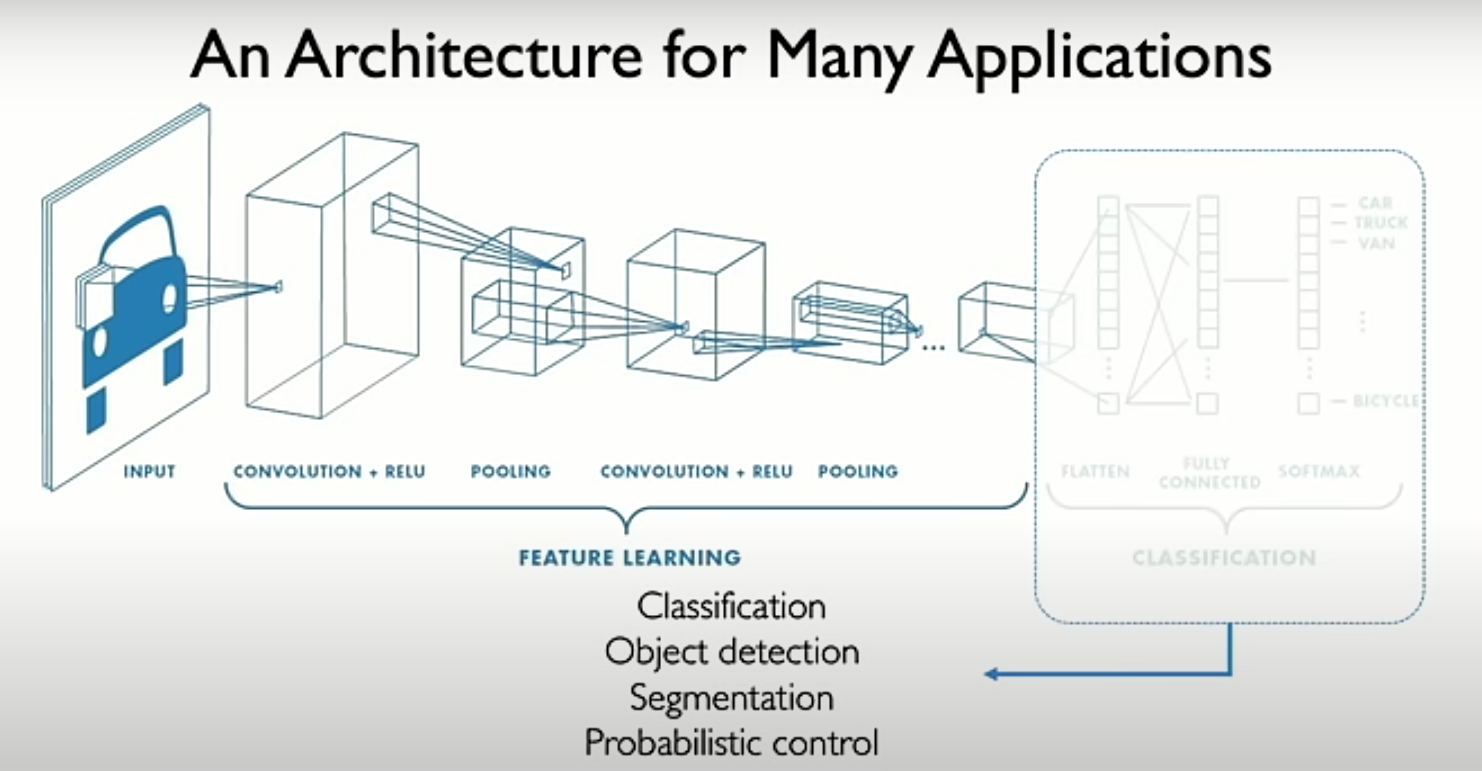
\includegraphics[width=\textwidth]{Images/cnn.png}
  \caption{CNN Architecture}
\end{figure}
\begin{itemize}
  \item We do this because deep in the layer we can then ignore the spatial structure, that is why we use flatten and then treat it as a regular fully connected neural network.
  \item So each box that yo see in the image is a collection of neurons, and each neuron is connected to a small region of the input image. And after many layers each neuron is connected to a small region in the filtered map of the previous layer.
  \item So we can see there is many applications for CNNs.
  \item So after the feature extraction we have so many possibilities, we can do whatever we want with the features, we can use them for classification, detection, segmentation, etc.
\end{itemize}
\begin{figure}[H]
  \centering
  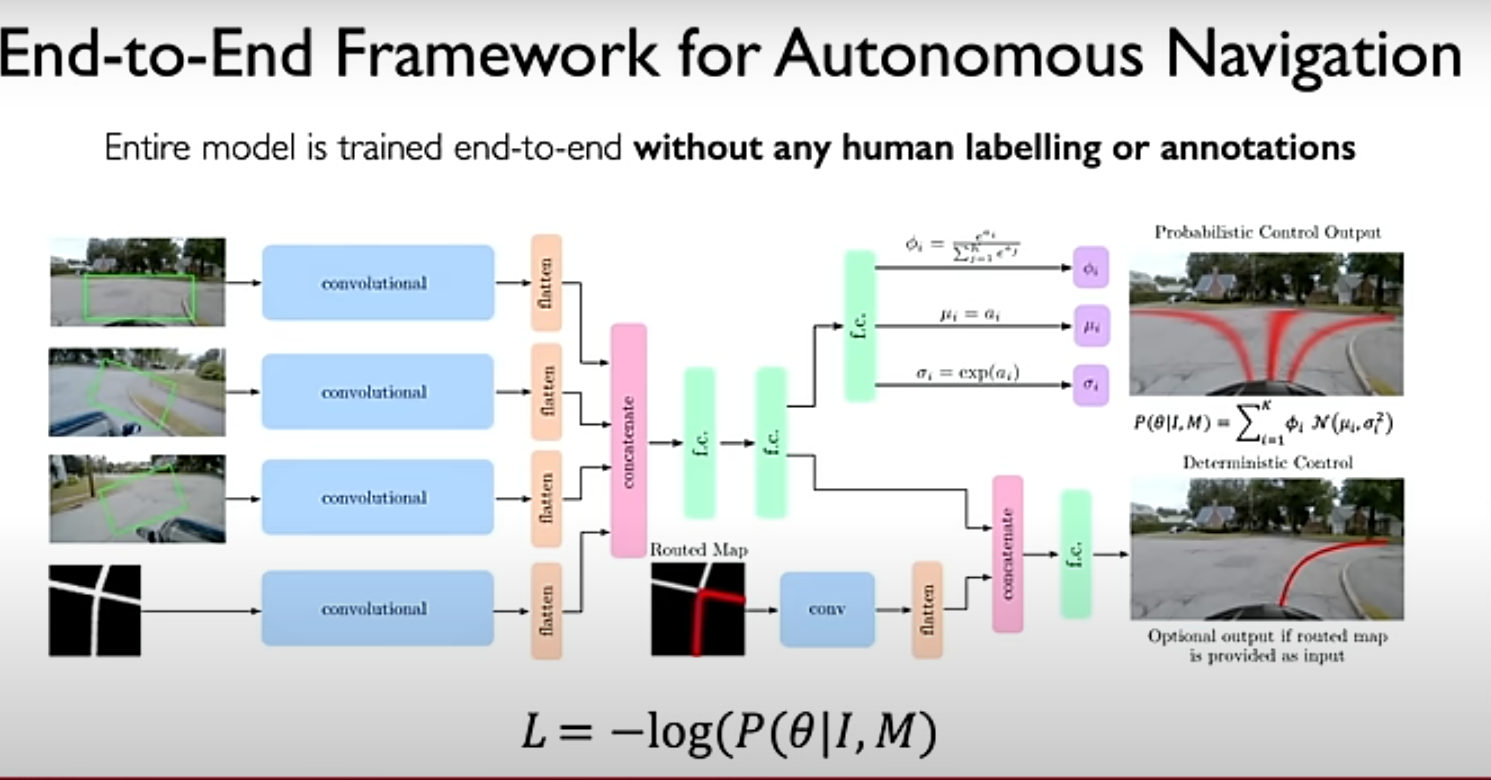
\includegraphics[width = \textwidth]{Images/cnn3.png}
  \caption{CNN example of self-driving car}
\end{figure}
\begin{itemize}
  \item F.c. means a fully connected network.
\end{itemize}
\begin{figure}[H]
  \centering
  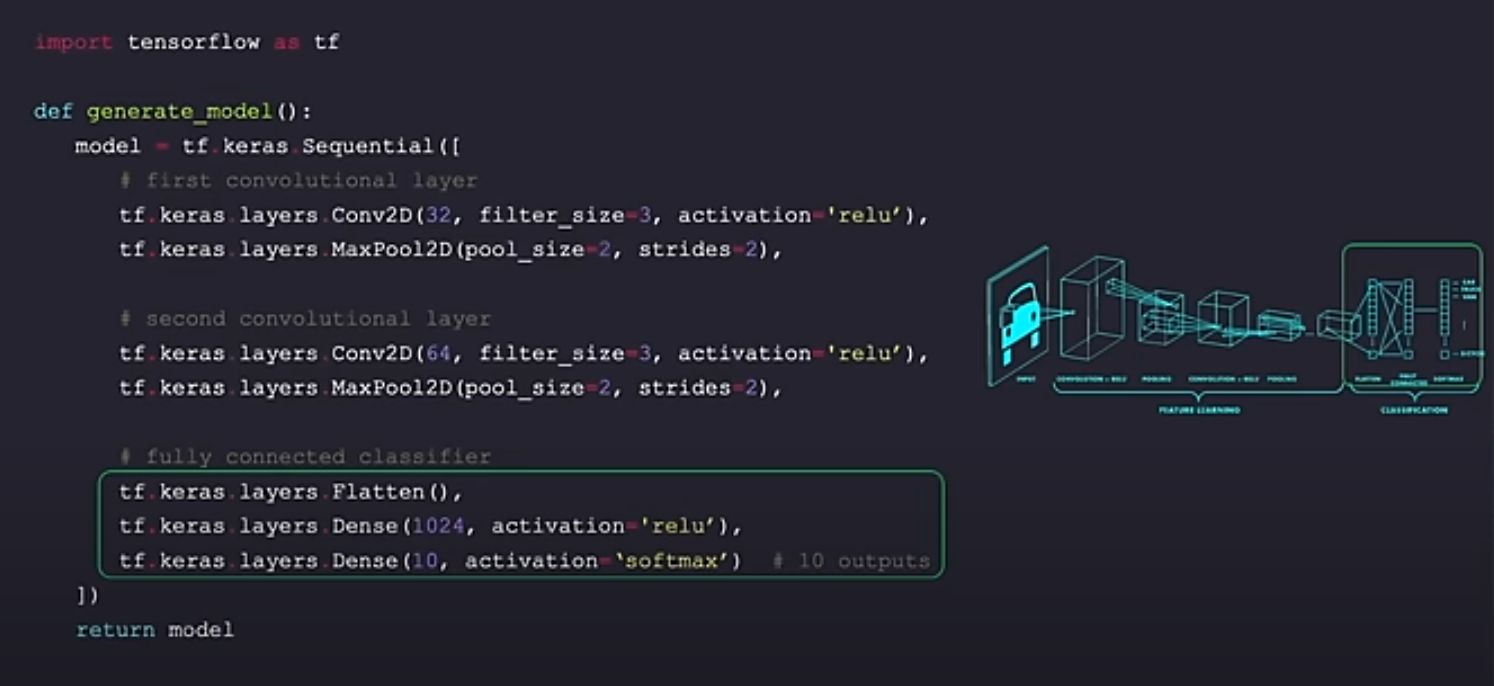
\includegraphics[width = \textwidth]{Images/cnn2.png}
  \caption{CNN Code Sample}
\end{figure}
\subsection*{How to actually solve the optimization problem? - Gradient Descent}
\begin{figure}[H]
  \centering
  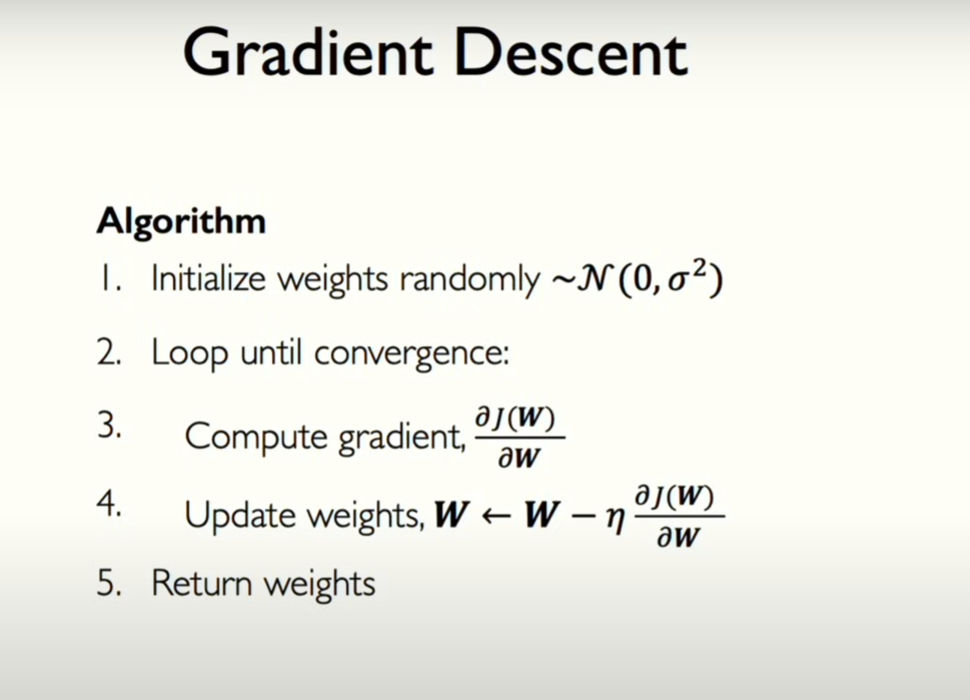
\includegraphics[width = \textwidth]{Images/gd.png}
  \caption{Gradient Descent}
\end{figure}
\begin{itemize}
  \item We can see that the learning rate is very important, if it is too small it will take a long time to converge, if it is too big it might overshoot the minimum.
  \item And we can see that if we choose a wrong initial value or a wrong learning rate we might get stuck in a local minimum.
\end{itemize}
\subsubsection*{To compute the gradient we use the chain rule(backpropagation)}
\begin{figure}[H]
  \centering
  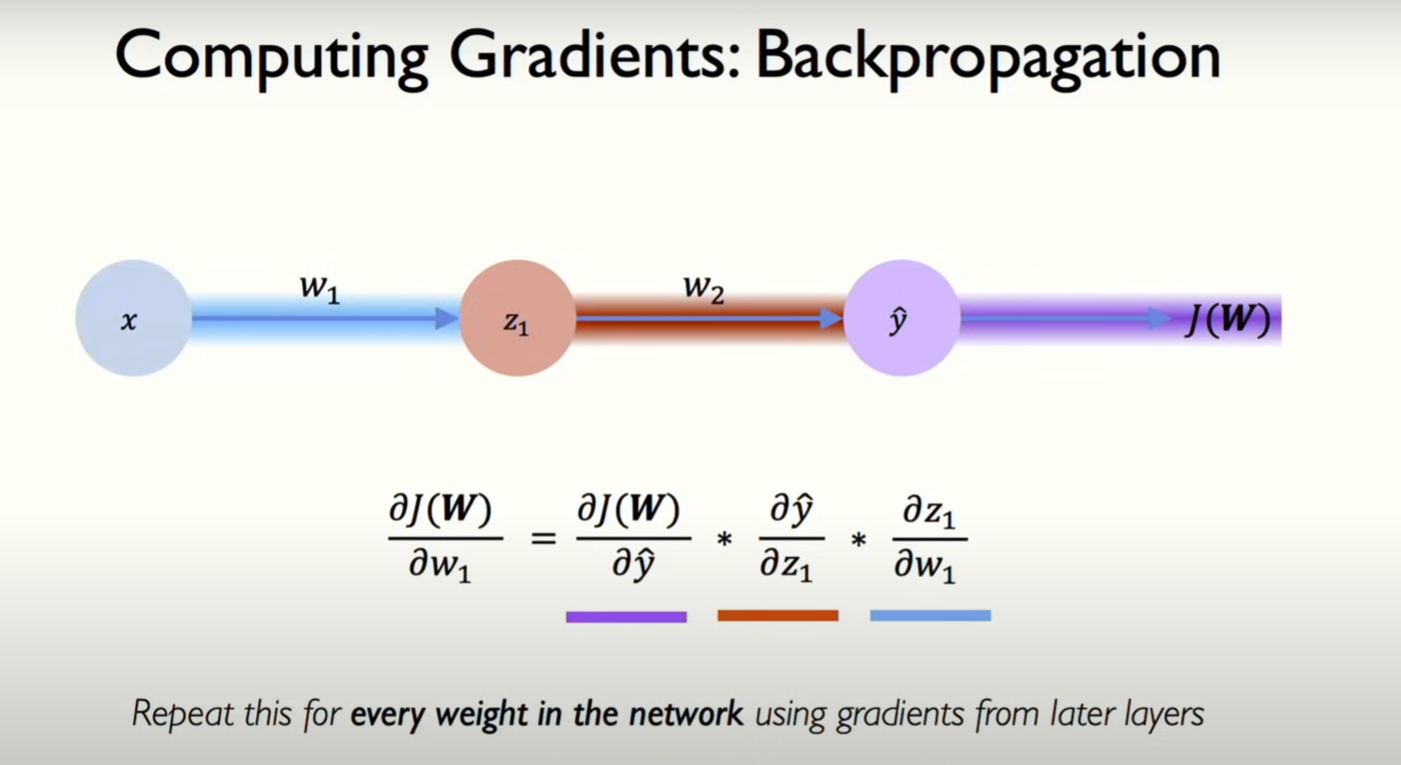
\includegraphics[width = \textwidth]{Images/backprop.png}
  \caption{Backpropagation}
\end{figure} 
\begin{itemize}
  \item You might be asking why we use backpropagation, why not just compute \(\frac{\partial J(W)}{\partial w_i}\)? Because the function $J(W)$ is a composition of functions, so we need to use the chain rule to compute the gradient. We can't directly compute the gradient with respect to $w_i$, instead, it's a complex function involving multiple layers of computation. Backpropagation, using the chain rule, allows us to correctly and efficiently compute this gradient by taking into account the entire chain of dependencies from $w_1$ to $J(W)$. (i.e. $J(W) \rightarrow \hat{y} \rightarrow z_1 \rightarrow w_1$)
\end{itemize}
In the end it all depends on the learning rate, so how do we choose this learning rate? One idea is to work with it as a hyperparameter, and try different values and see which one works best. Another idea is to use adaptive learning rates!!
\subsubsection*{Adaptive Learning Rates - Optimizing Gradient Descent}
\begin{itemize}
  \item Adagrad: It adapts the learning rate to the parameters, so it gives a different learning rate to each parameter. It is good for sparse data.
  \item RMSprop: It is similar to Adagrad, but it divides the learning rate by the square root of the sum of the squares of the gradients. It is good for non-stationary data.
  \item Adam: It is a combination of RMSprop and momentum. It is good for large datasets and high-dimensional data.
  \item SGD: Stochastic Gradient Descent, it is the most basic one, it is good for large datasets. ( we chose a random batch (sample of the data) and we compute the gradient on this batch and we update the weights, and we repeat this process until we reach the minimum ).
  \begin{figure}[H]
    \centering
    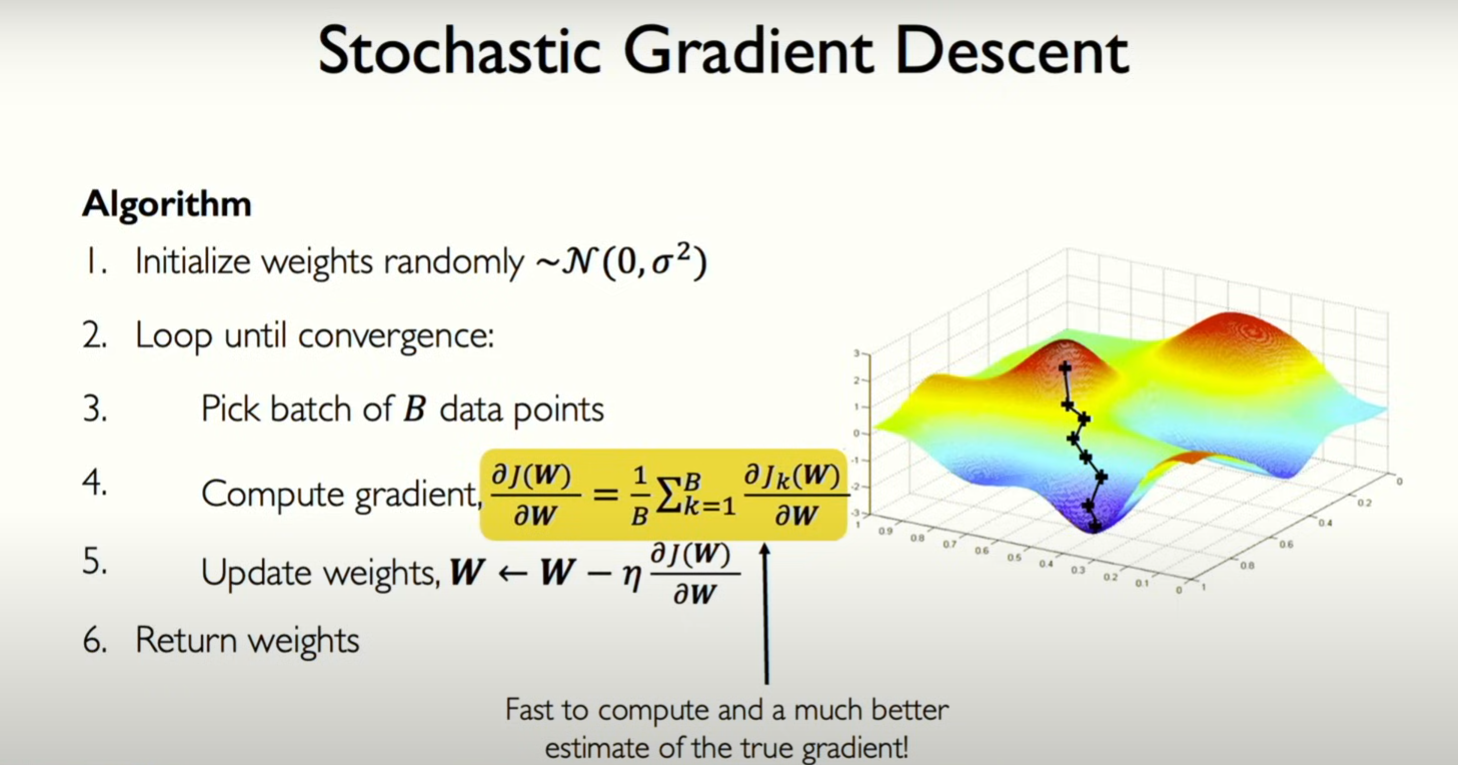
\includegraphics[width = \textwidth]{Images/SGD.png}
    \caption{SGD}
  \end{figure}
\end{itemize}
\subsubsection*{\underline{How to apply regularization?}}
\subsubsection{Dropout}
\begin{itemize}
  \item During training set some activations to 0, typically 50\% of the activations are set to 0, which forces the network to not rely on a single neuron. $tf.keras.layers.Dropout(p=0.5)$
\end{itemize}
\subsubsection{Early Stopping}
\begin{itemize}
  \item We stop training when the test error starts to increase, because this means that the model is overfitting. (find the sweet spot between underfitting and overfitting)
\end{itemize}
\subsection*{Sequence Models}
\subsubsection*{RNN - Recurrent Neural Networks}
\begin{figure}[H]
  \centering
  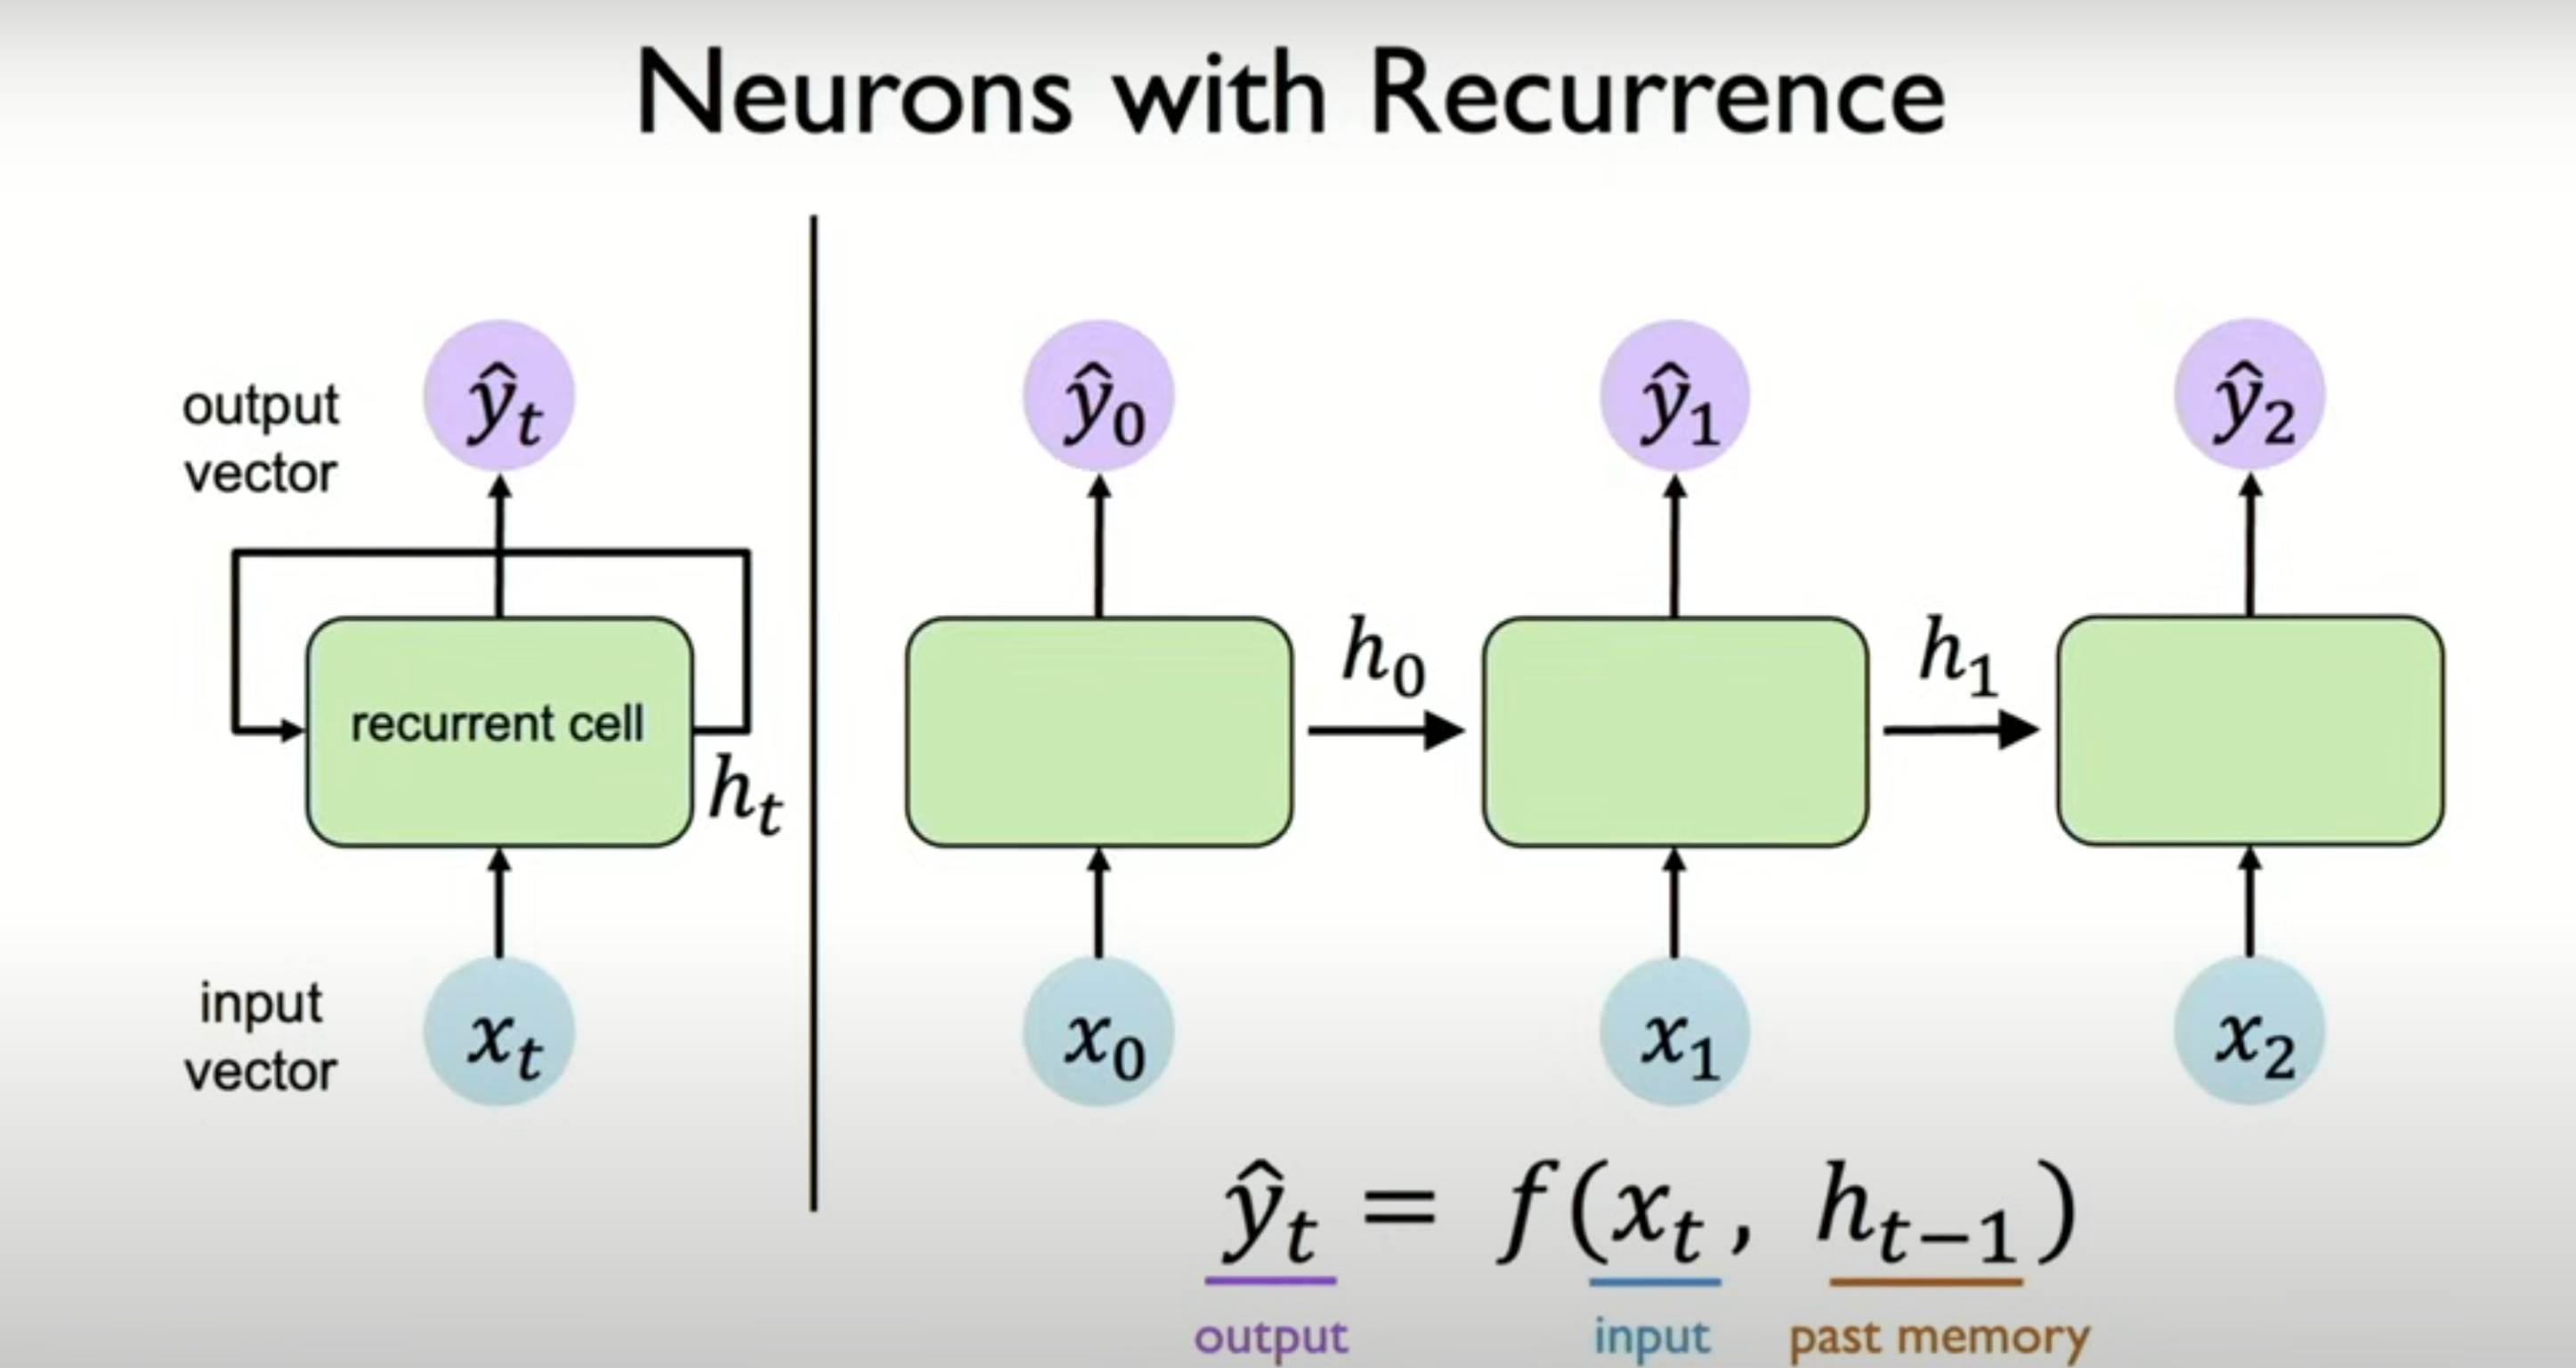
\includegraphics[width = \textwidth]{Images/rnn.png}
  \caption{RNN}
\end{figure}
\begin{itemize}
  \item RNNs is the foundation of sequence models.
  \item They are used for sequence data, like time series, text, etc.
  \item The figure above help us understand the Architecture of an RNN.
  \item So what you see is that on the right this is ultimately what we are doing, but we don't have many models, so think about it as a recursion, so it is re going back to itself on the next input, so it is like a loop. Which we can see from the diagram on the left. This means that at time equal t we are using the information from time = t-1, modeled by $h_{t-1}$, and the input $x_t$ at this particular time.
  \item Now let's formalize this a bit more, not that in the figure below we are modifying the weights as we go along the sequence, so we are not using the same weights for all the inputs, we are using the same weights but we are modifying them as we go along the sequence.
  
  \begin{figure}[H]
    \centering
    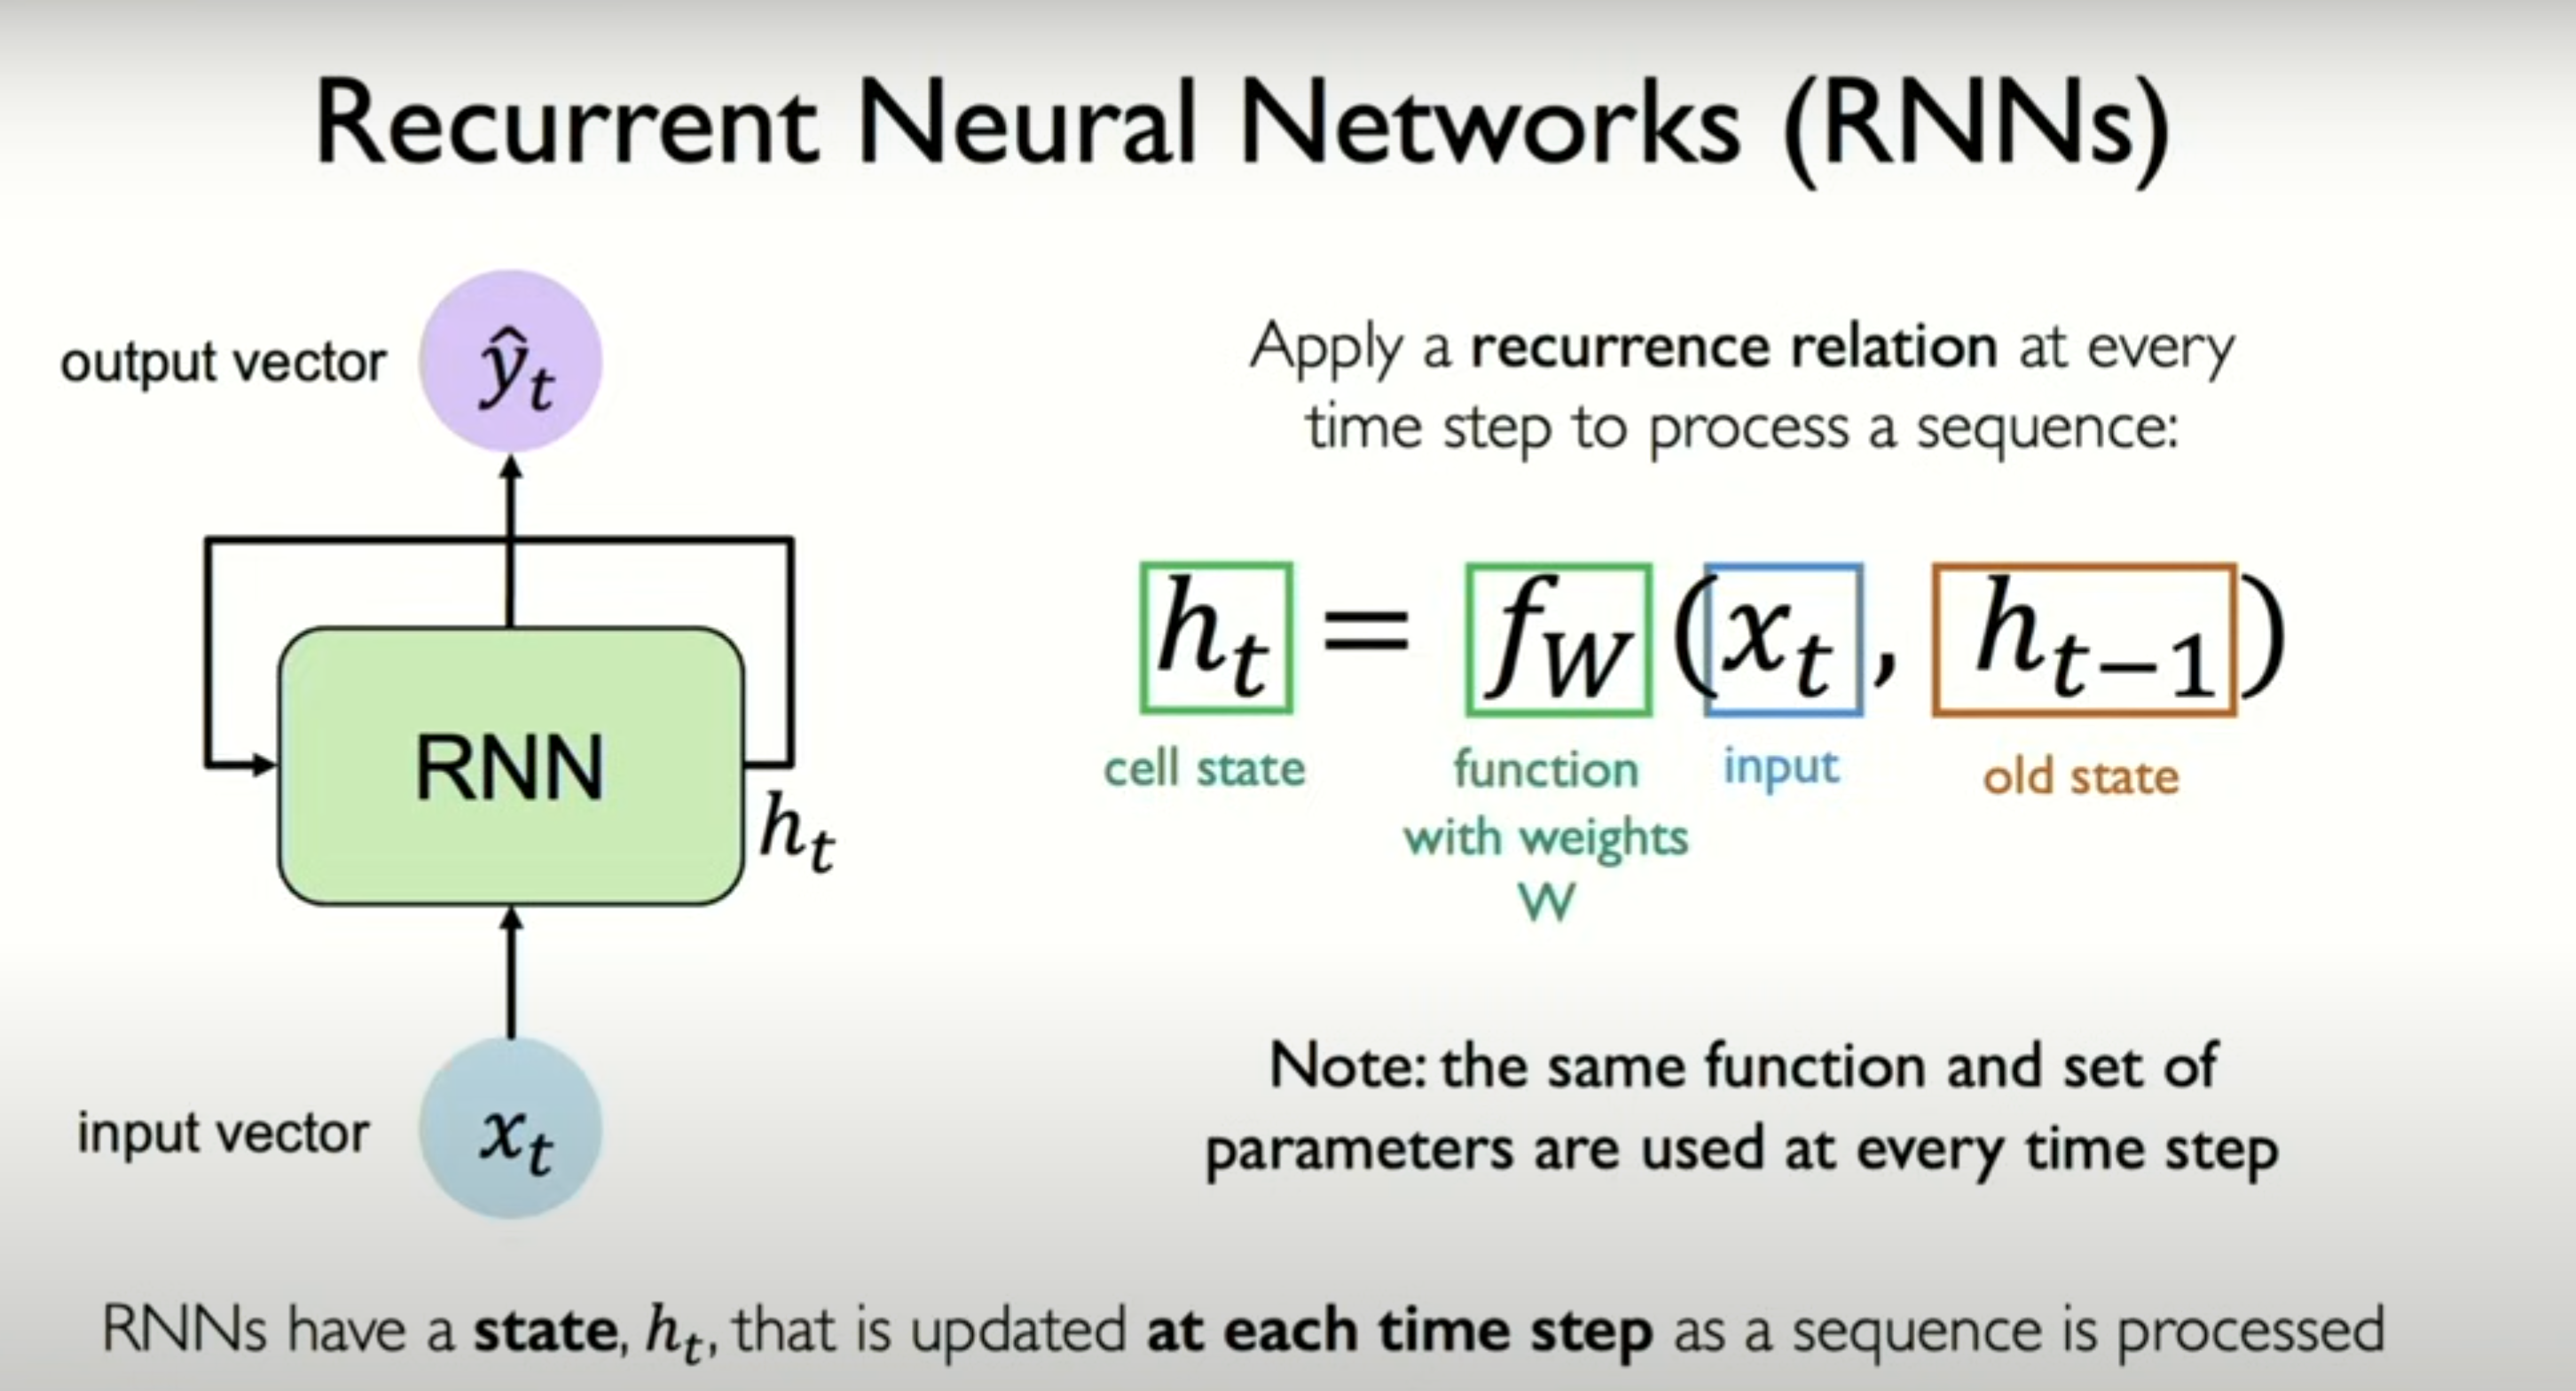
\includegraphics[width = \textwidth]{Images/rnn2.png}
    \caption{RNN Formalization}
  \end{figure}

  \begin{figure}[H]
    \centering
    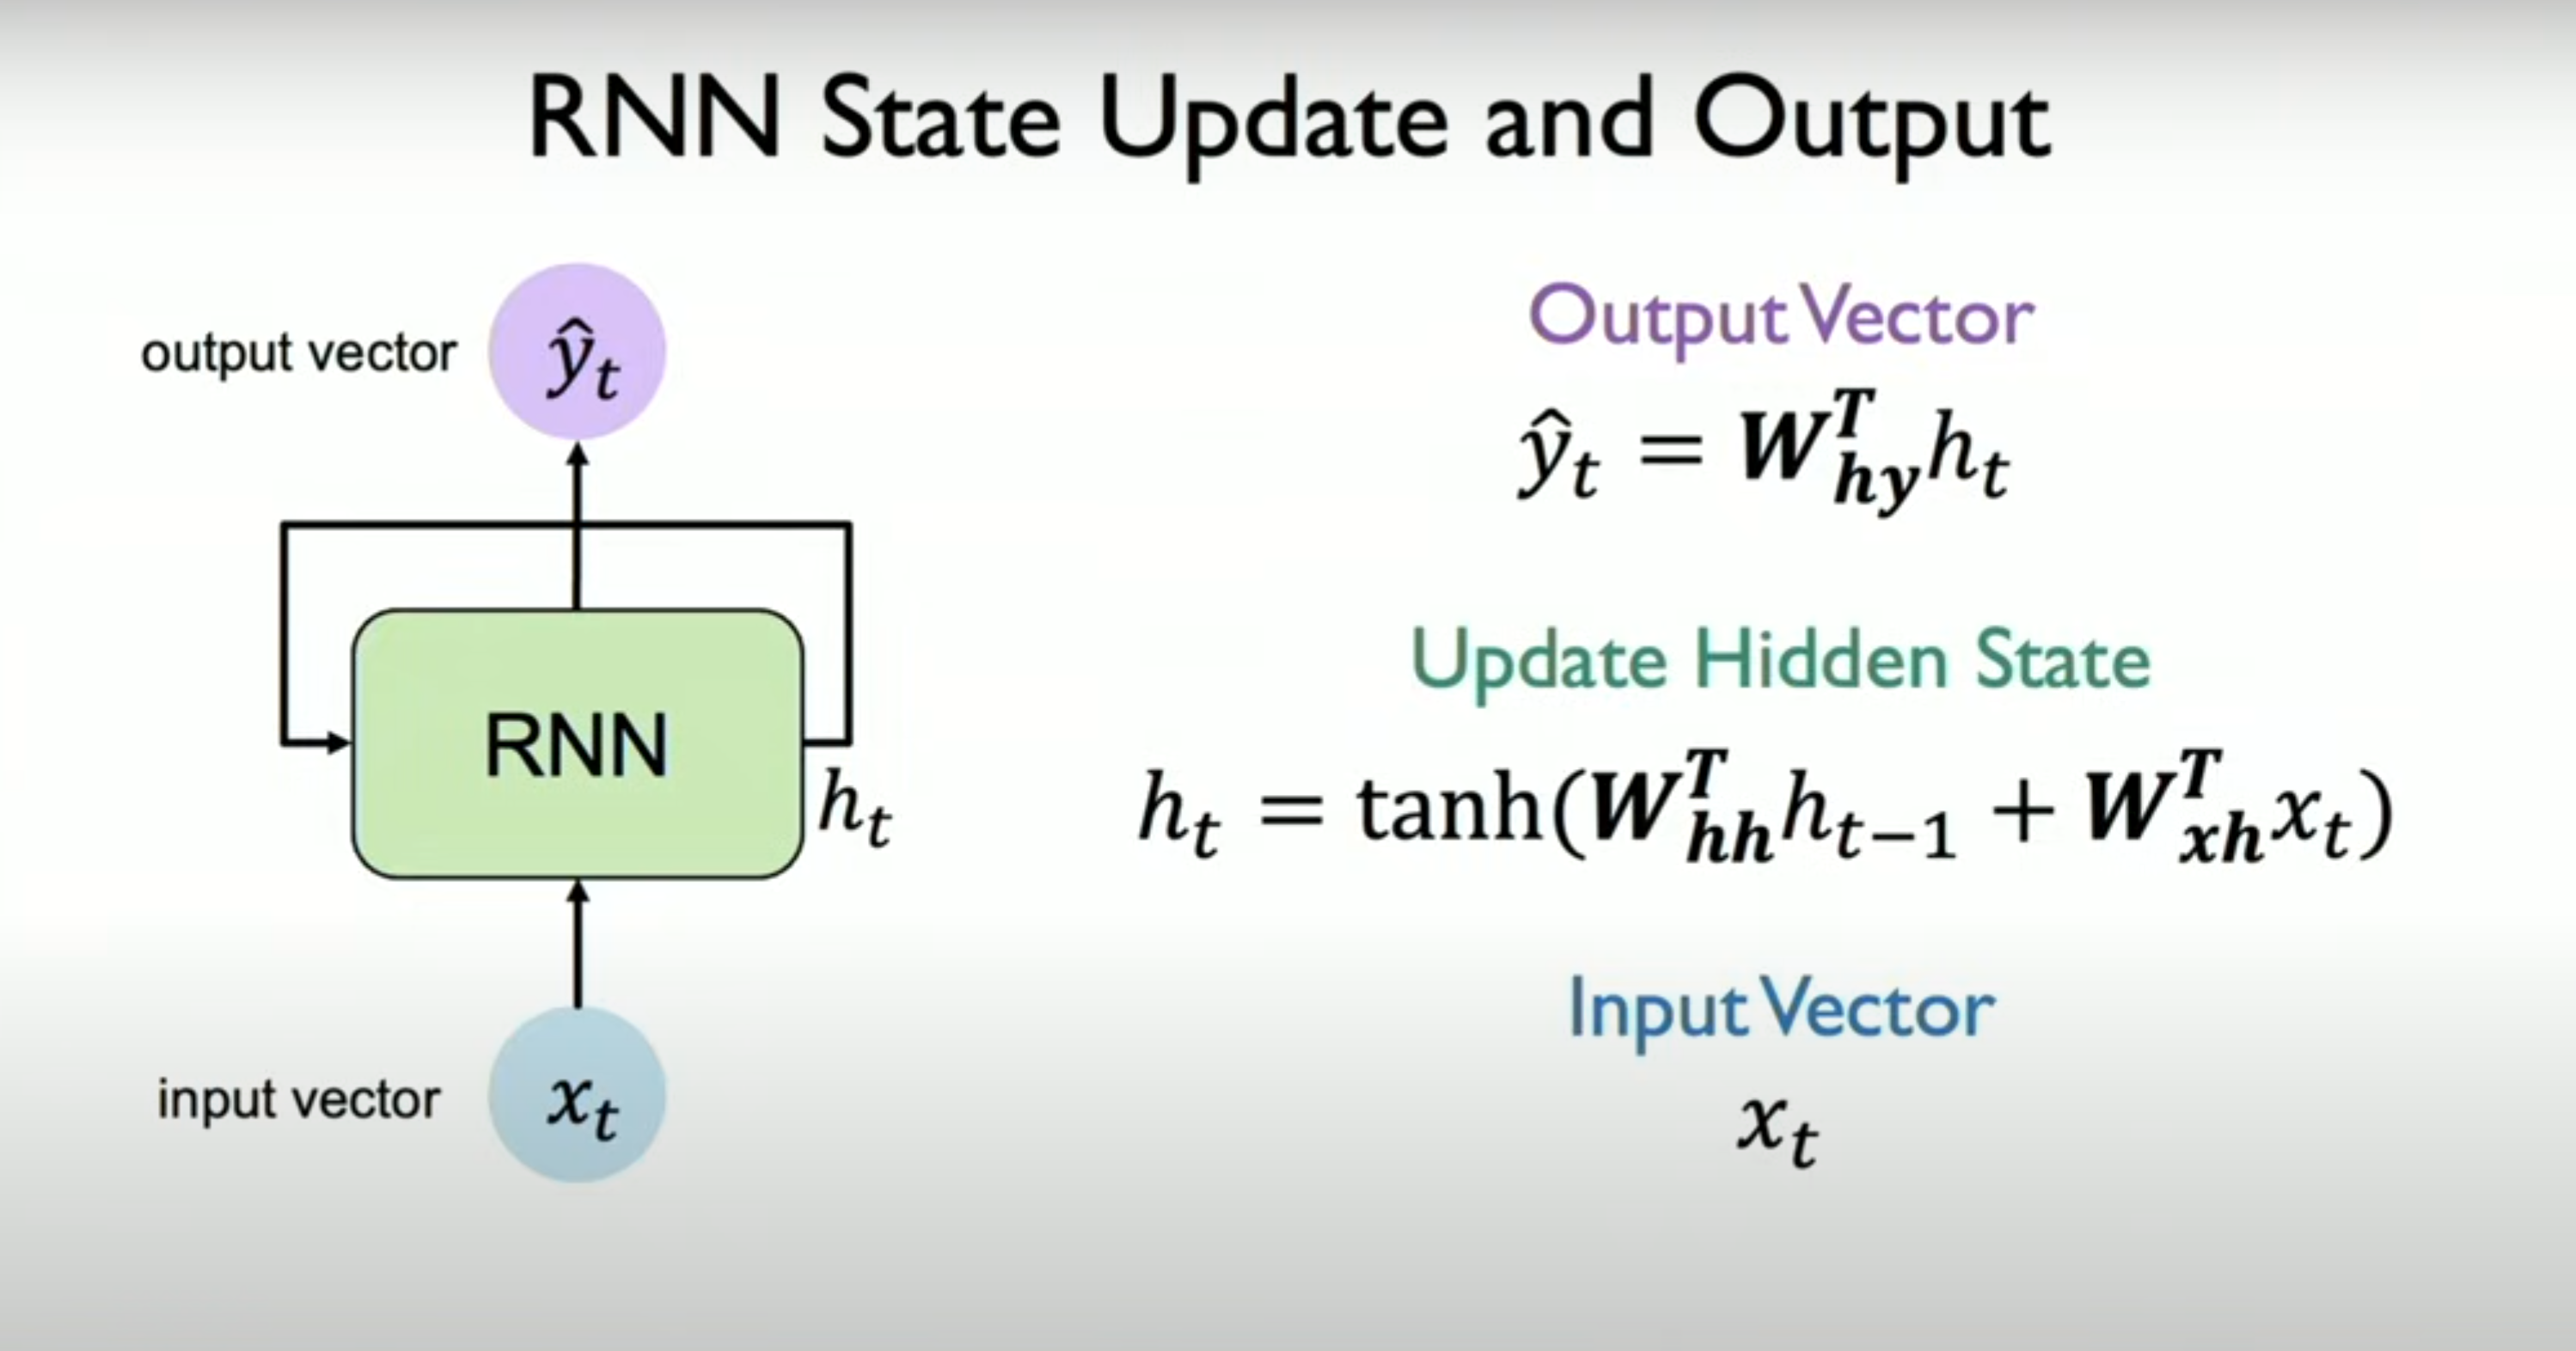
\includegraphics[width = \textwidth]{Images/rnn5.png}
    \caption{RNN- Across time steps (1)}
  \end{figure}
    \begin{figure}[H]
      \centering
      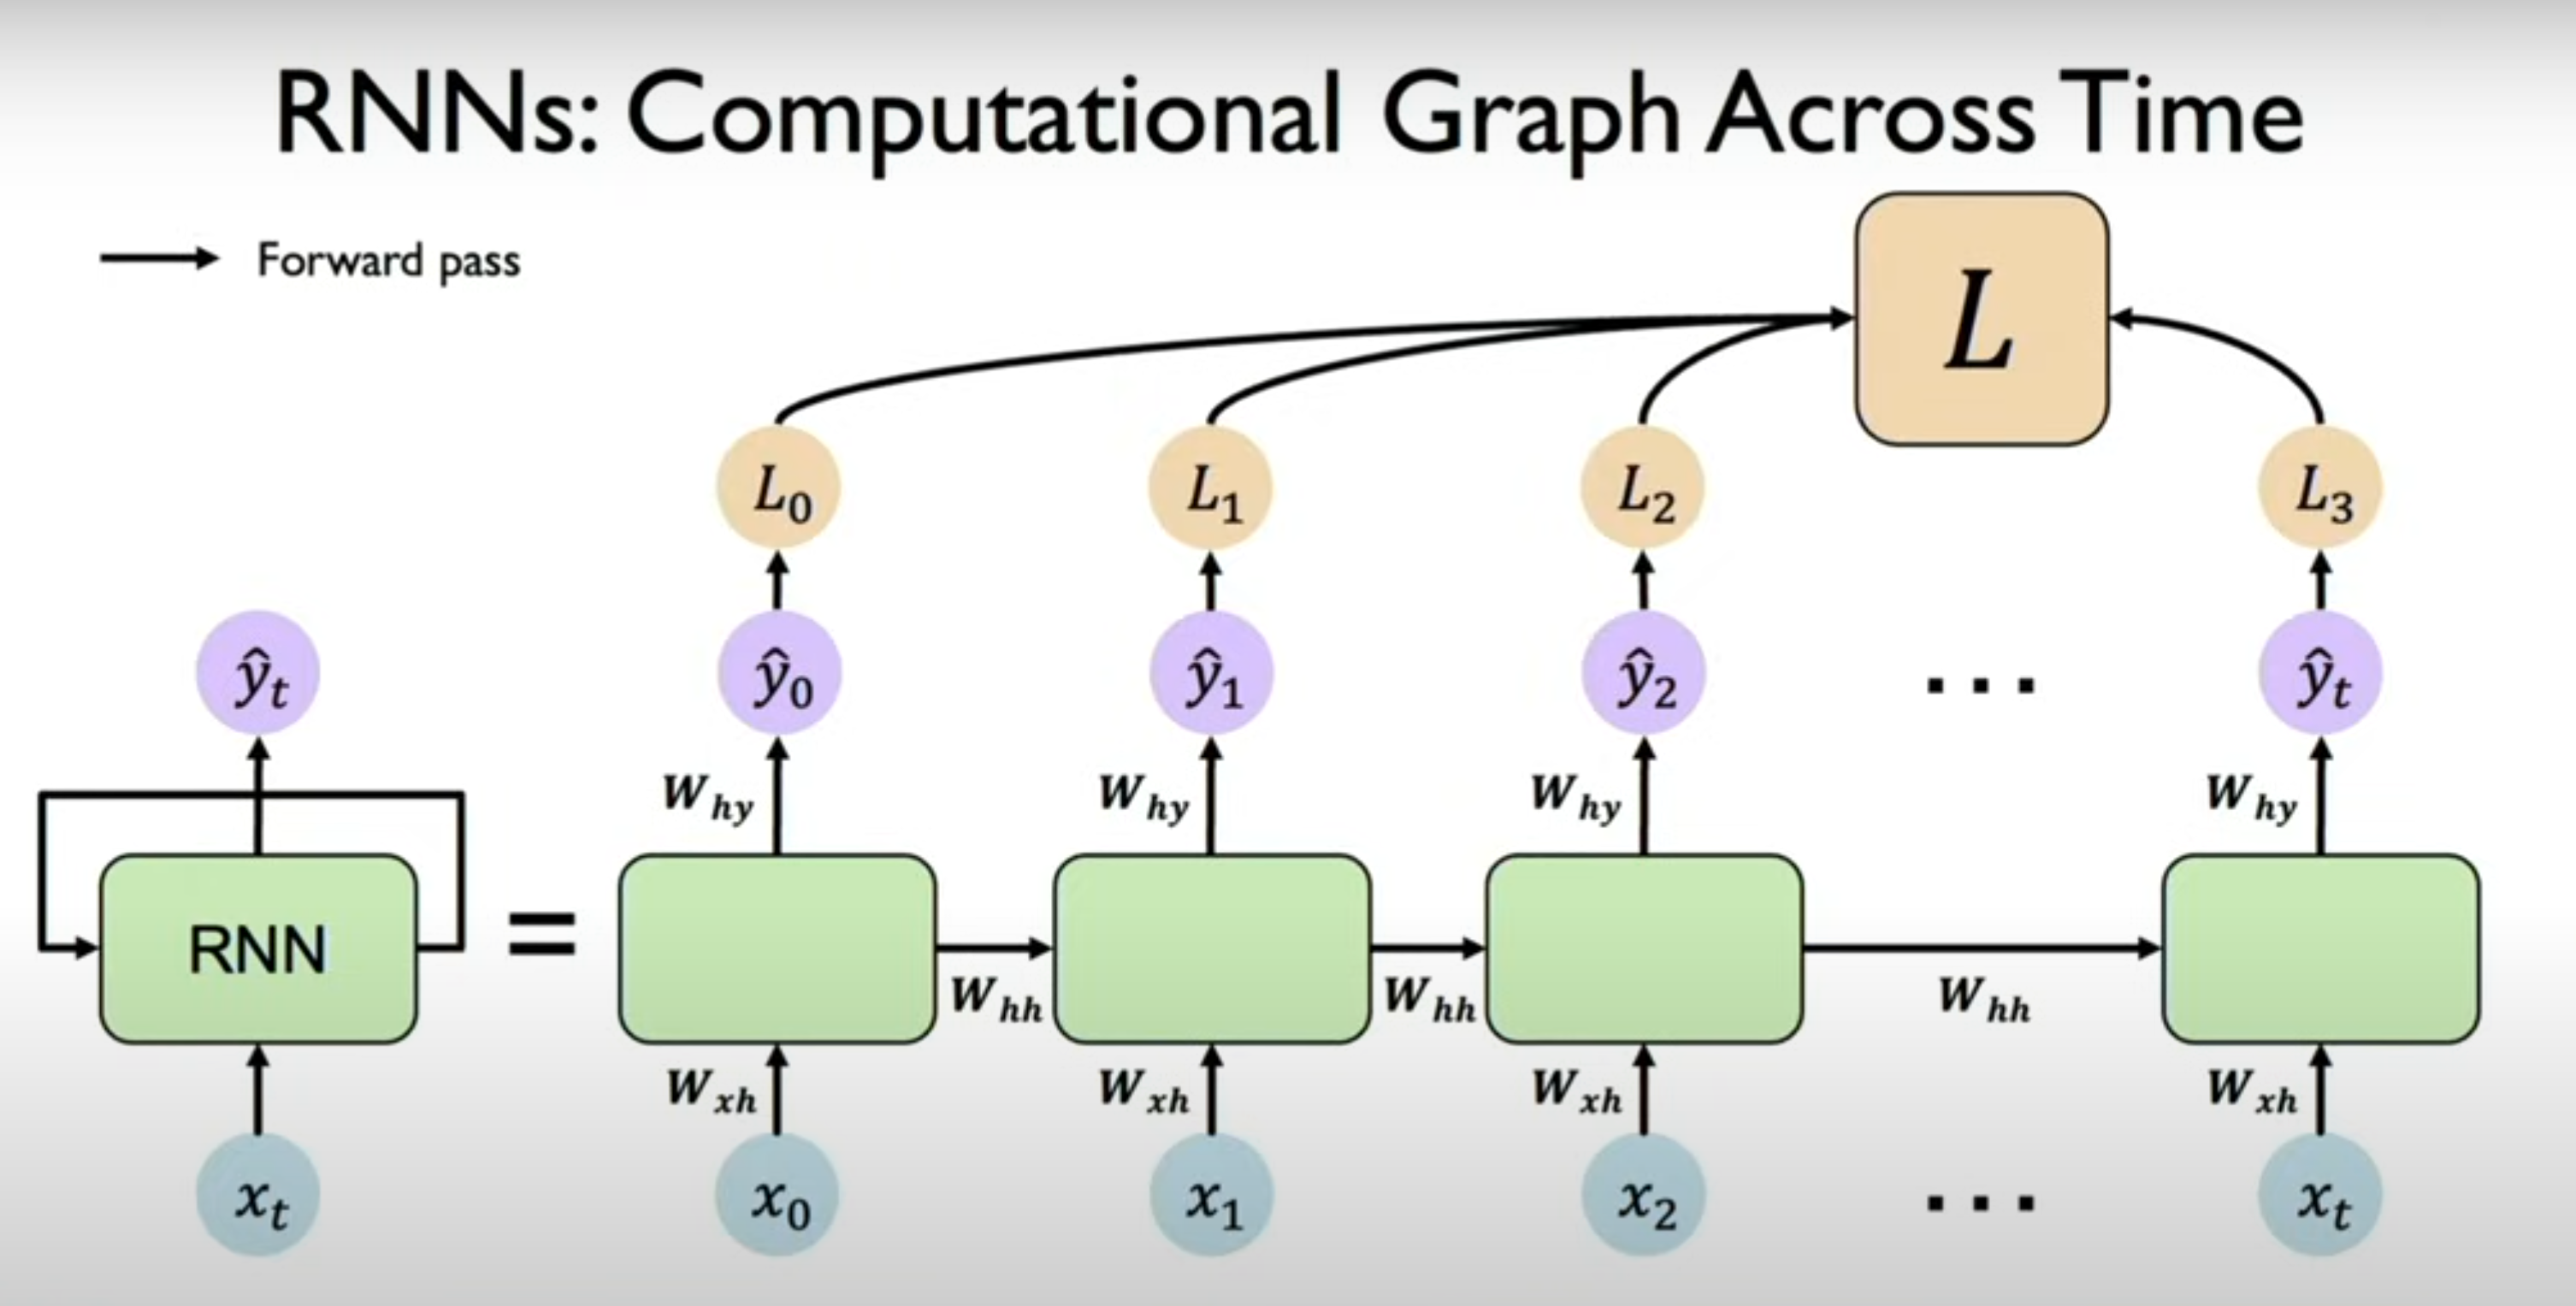
\includegraphics[width = \textwidth]{Images/rnn4.png}
      \caption{RNN- Across time steps (2)}
    \end{figure}
    \item The $L_i$ are then summed up to get the final loss $L$.
    \item The weights matrices are the same matrices but are being updated as we go along the sequence.
    \item We can see that $\hat{y}_t = W_{hy}^Th_{t}$
    \item The weights are shared across the sequence.
    \item The weights are updated using backpropagation through time.
    \begin{figure}[H]
      \centering
      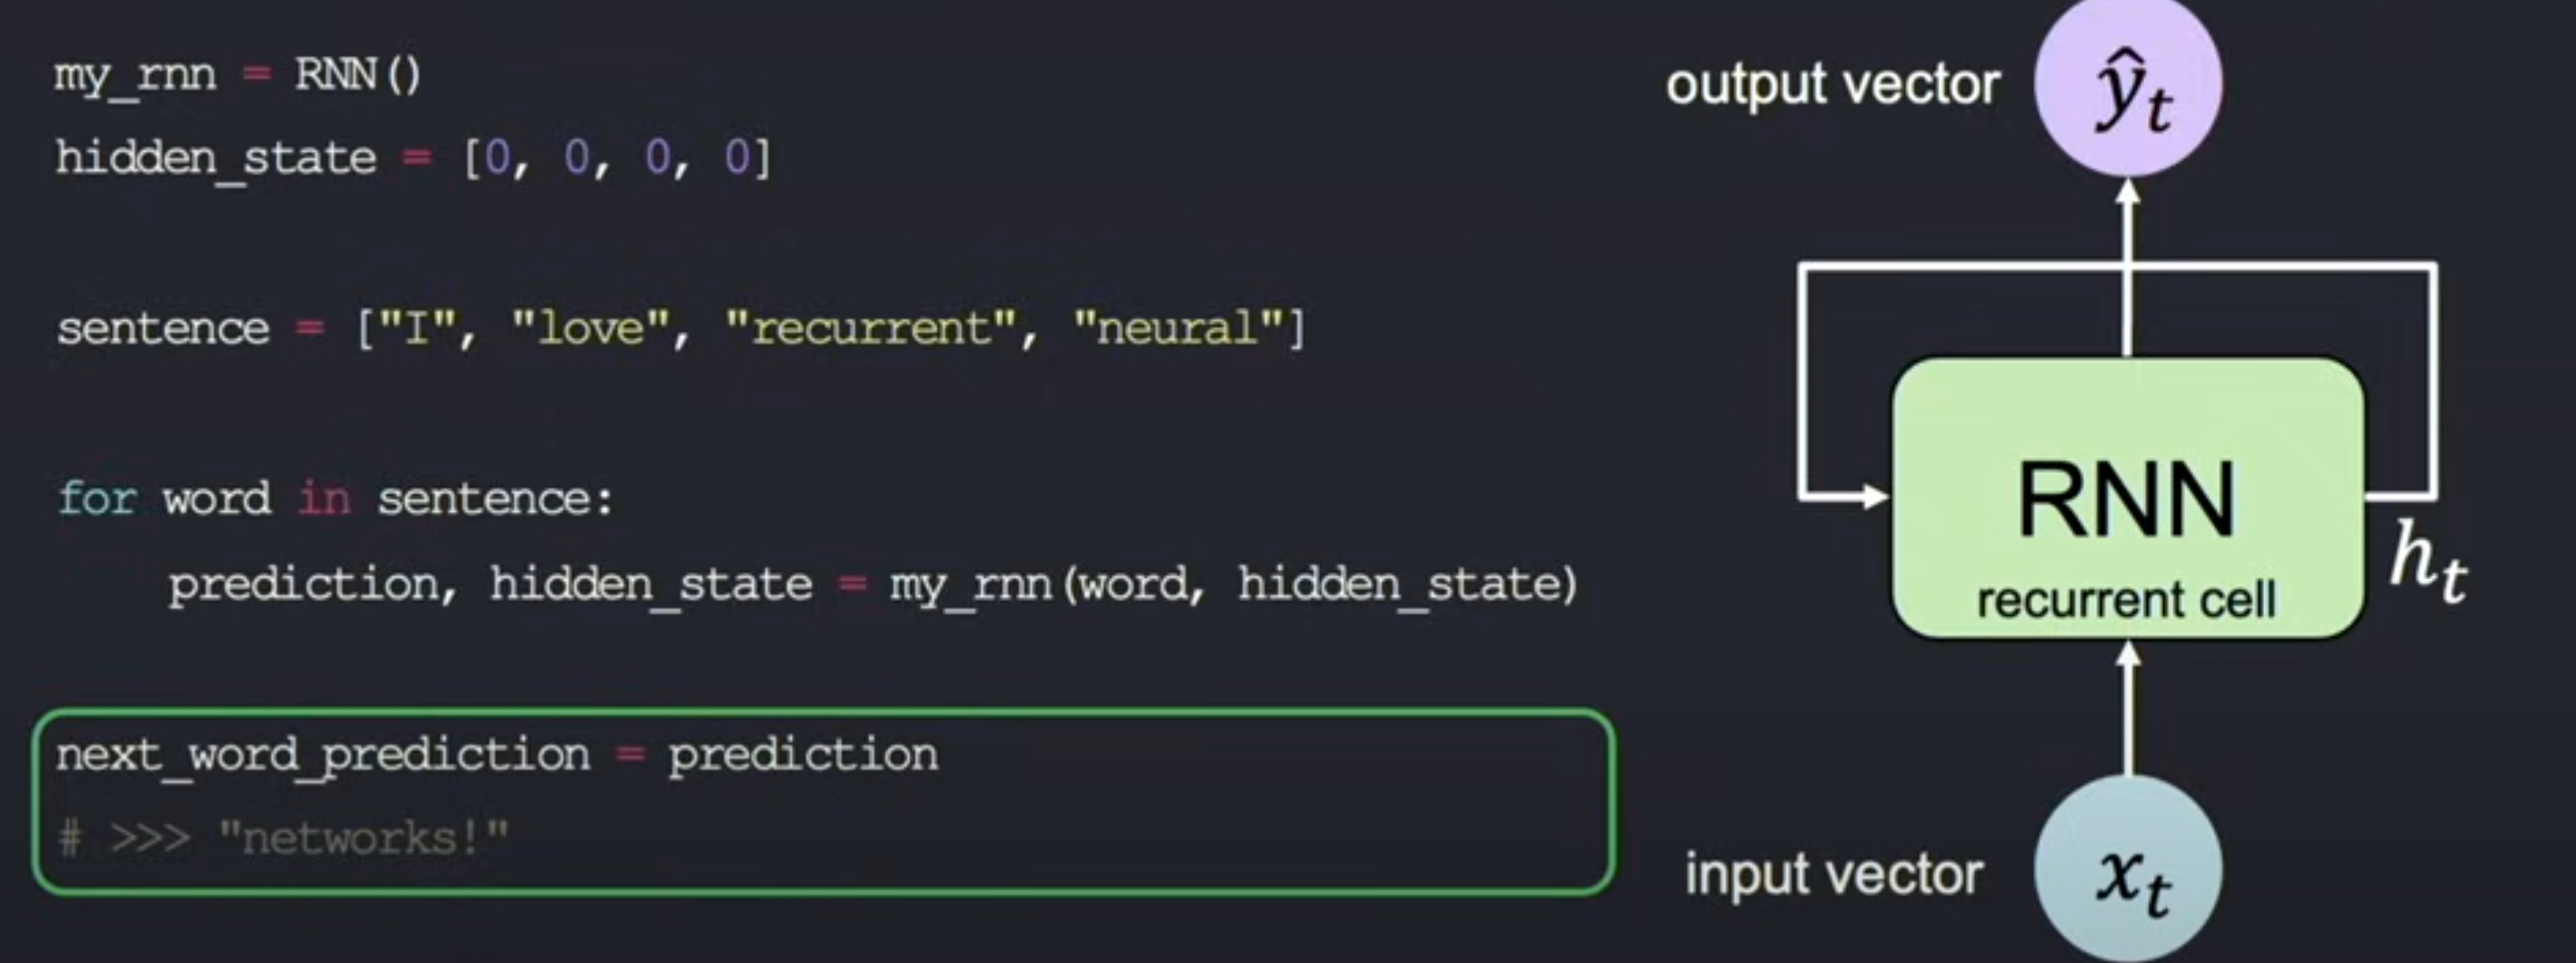
\includegraphics[width = \textwidth]{Images/rnn3.png}
      \caption{RNN Code Sample - to easily visualize the architecture}
    \end{figure}
    \begin{figure}[H]
      \centering
      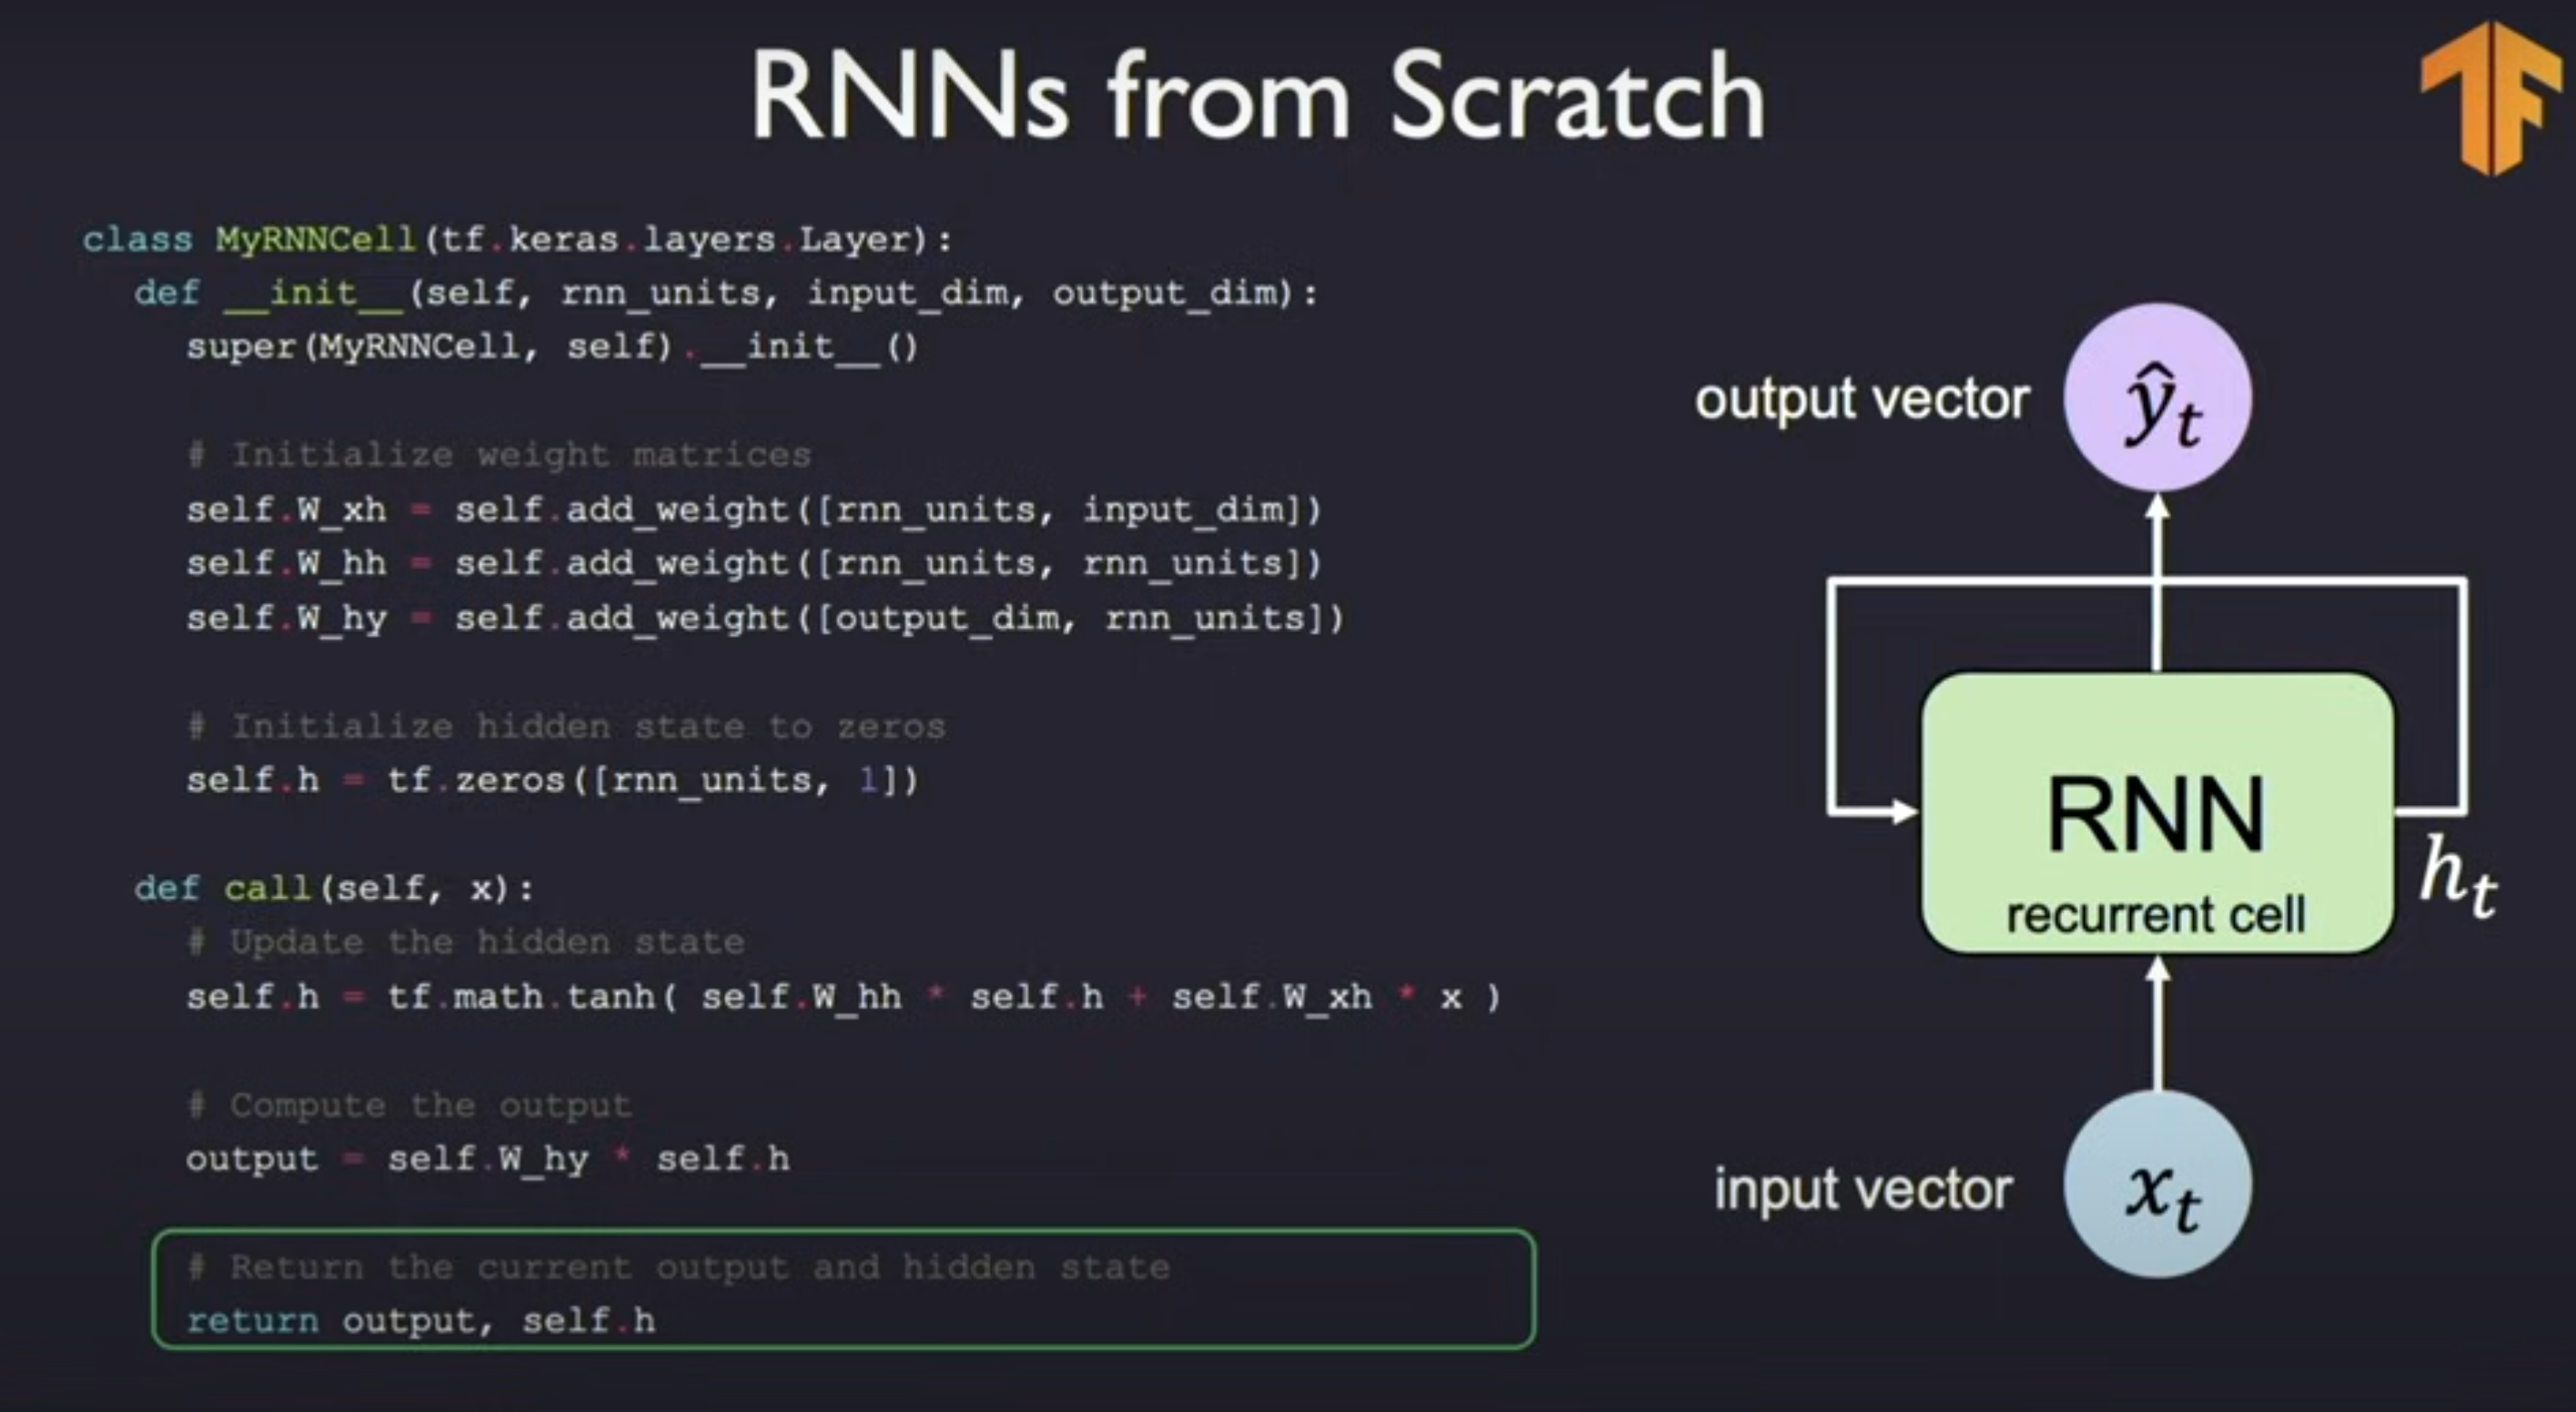
\includegraphics[width = \textwidth]{Images/rnn6.png}
      \caption{RNN Code from Scratch - to understand the architecture}
    \end{figure}
    \item  Instead of this you just use $tf.keras.layers.SimpleRNN(rnn\_units)$
\end{itemize}
\subsubsection*{Example of A Sequence Modeling Problem: \underline{Predict the next word}}
\begin{itemize}
  \item We need to make sure of handling variable-length sequences.
  \item Track long-term dependencies.
  \item Maintain the order of the sequence.
  \item Share parameters across the sequence. 
  \item Fortunately, RNNs can handle all of these requirements(some more than others).
  \item First Question, that we might ask ourselves is that: How do we represent the words? How should we encode language? 
  \end{itemize}
  \subsubsection{One-Hot Encoding}
  \begin{itemize}
    \item Like a lookup table, so we have a vector of zeros and a 1 at the index of the word. The length of the vector is the size of the vocabulary.
  \end{itemize}
  \subsubsection{Word Embeddings}
  \begin{itemize}
    \item Learned Embedding, you might ask what dimension of the embedding we use? 
    \item You might think at first that as the number of distinct things in my vocab increases, we should always increase the dimension of the embedding, but this is not the case, we need to find a sweet spot, because if we increase the dimension too much we lose the point of the embedding, which is to capture the semantic meaning of the words, and we might then end up with a sparse representation, which is not what we want (i.e. similar to one-Hot embedding). 
    \item Sparse Categorical Crossentropy: This is used when your labels are integers representing class indices, rather than one-hot encoded vectors. If you have a vocabulary of size 1000, for instance, your labels will be integers from 0 to 999. $tf.keras.losses.sparse_categorical_crossentropy$
    \item Categorical Crossentropy Loss Crossentropy: A measure of the difference between two probability distributions. In the context of classification, it's a measure of how well the predicted probability distribution (after softmax) matches the true distribution (represented by the labels).
  \end{itemize}
  \subsubsection*{Now How do we train the model?}
  \begin{figure}[H]
    \centering
    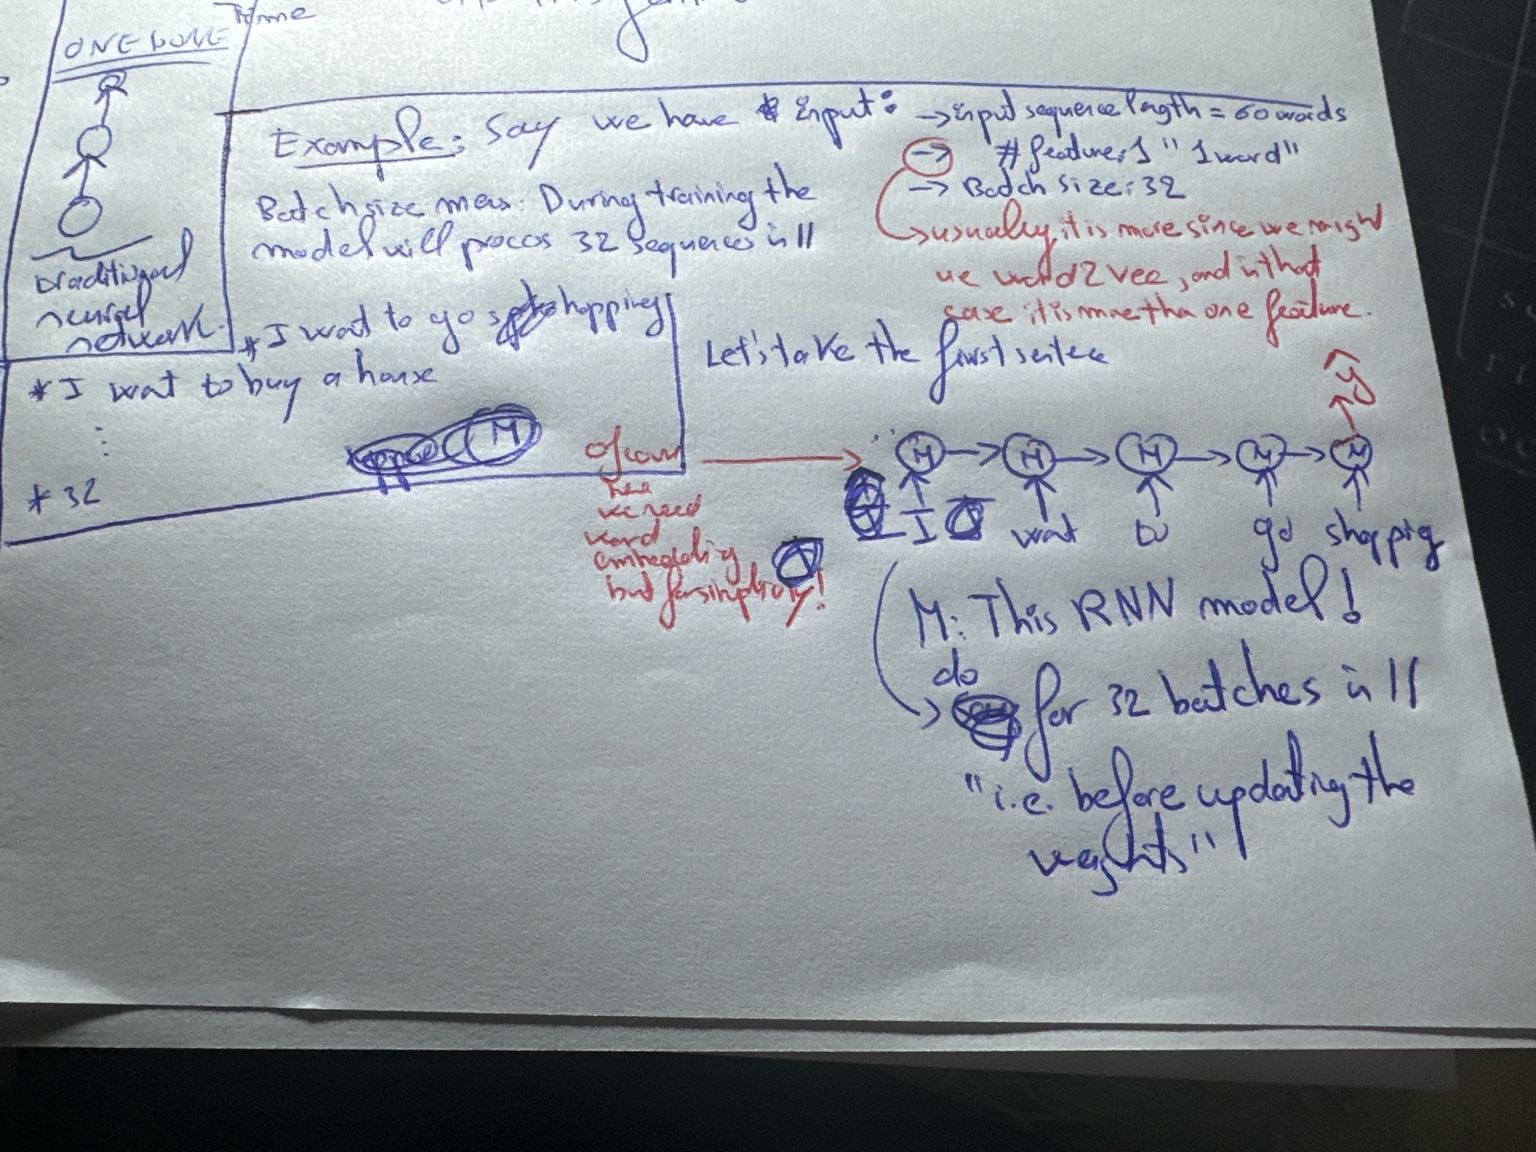
\includegraphics[width = \textwidth]{Images/RNN_SKETCH.jpeg}
    \caption{Training the Model}
  \end{figure}
  \begin{figure}
    \centering
    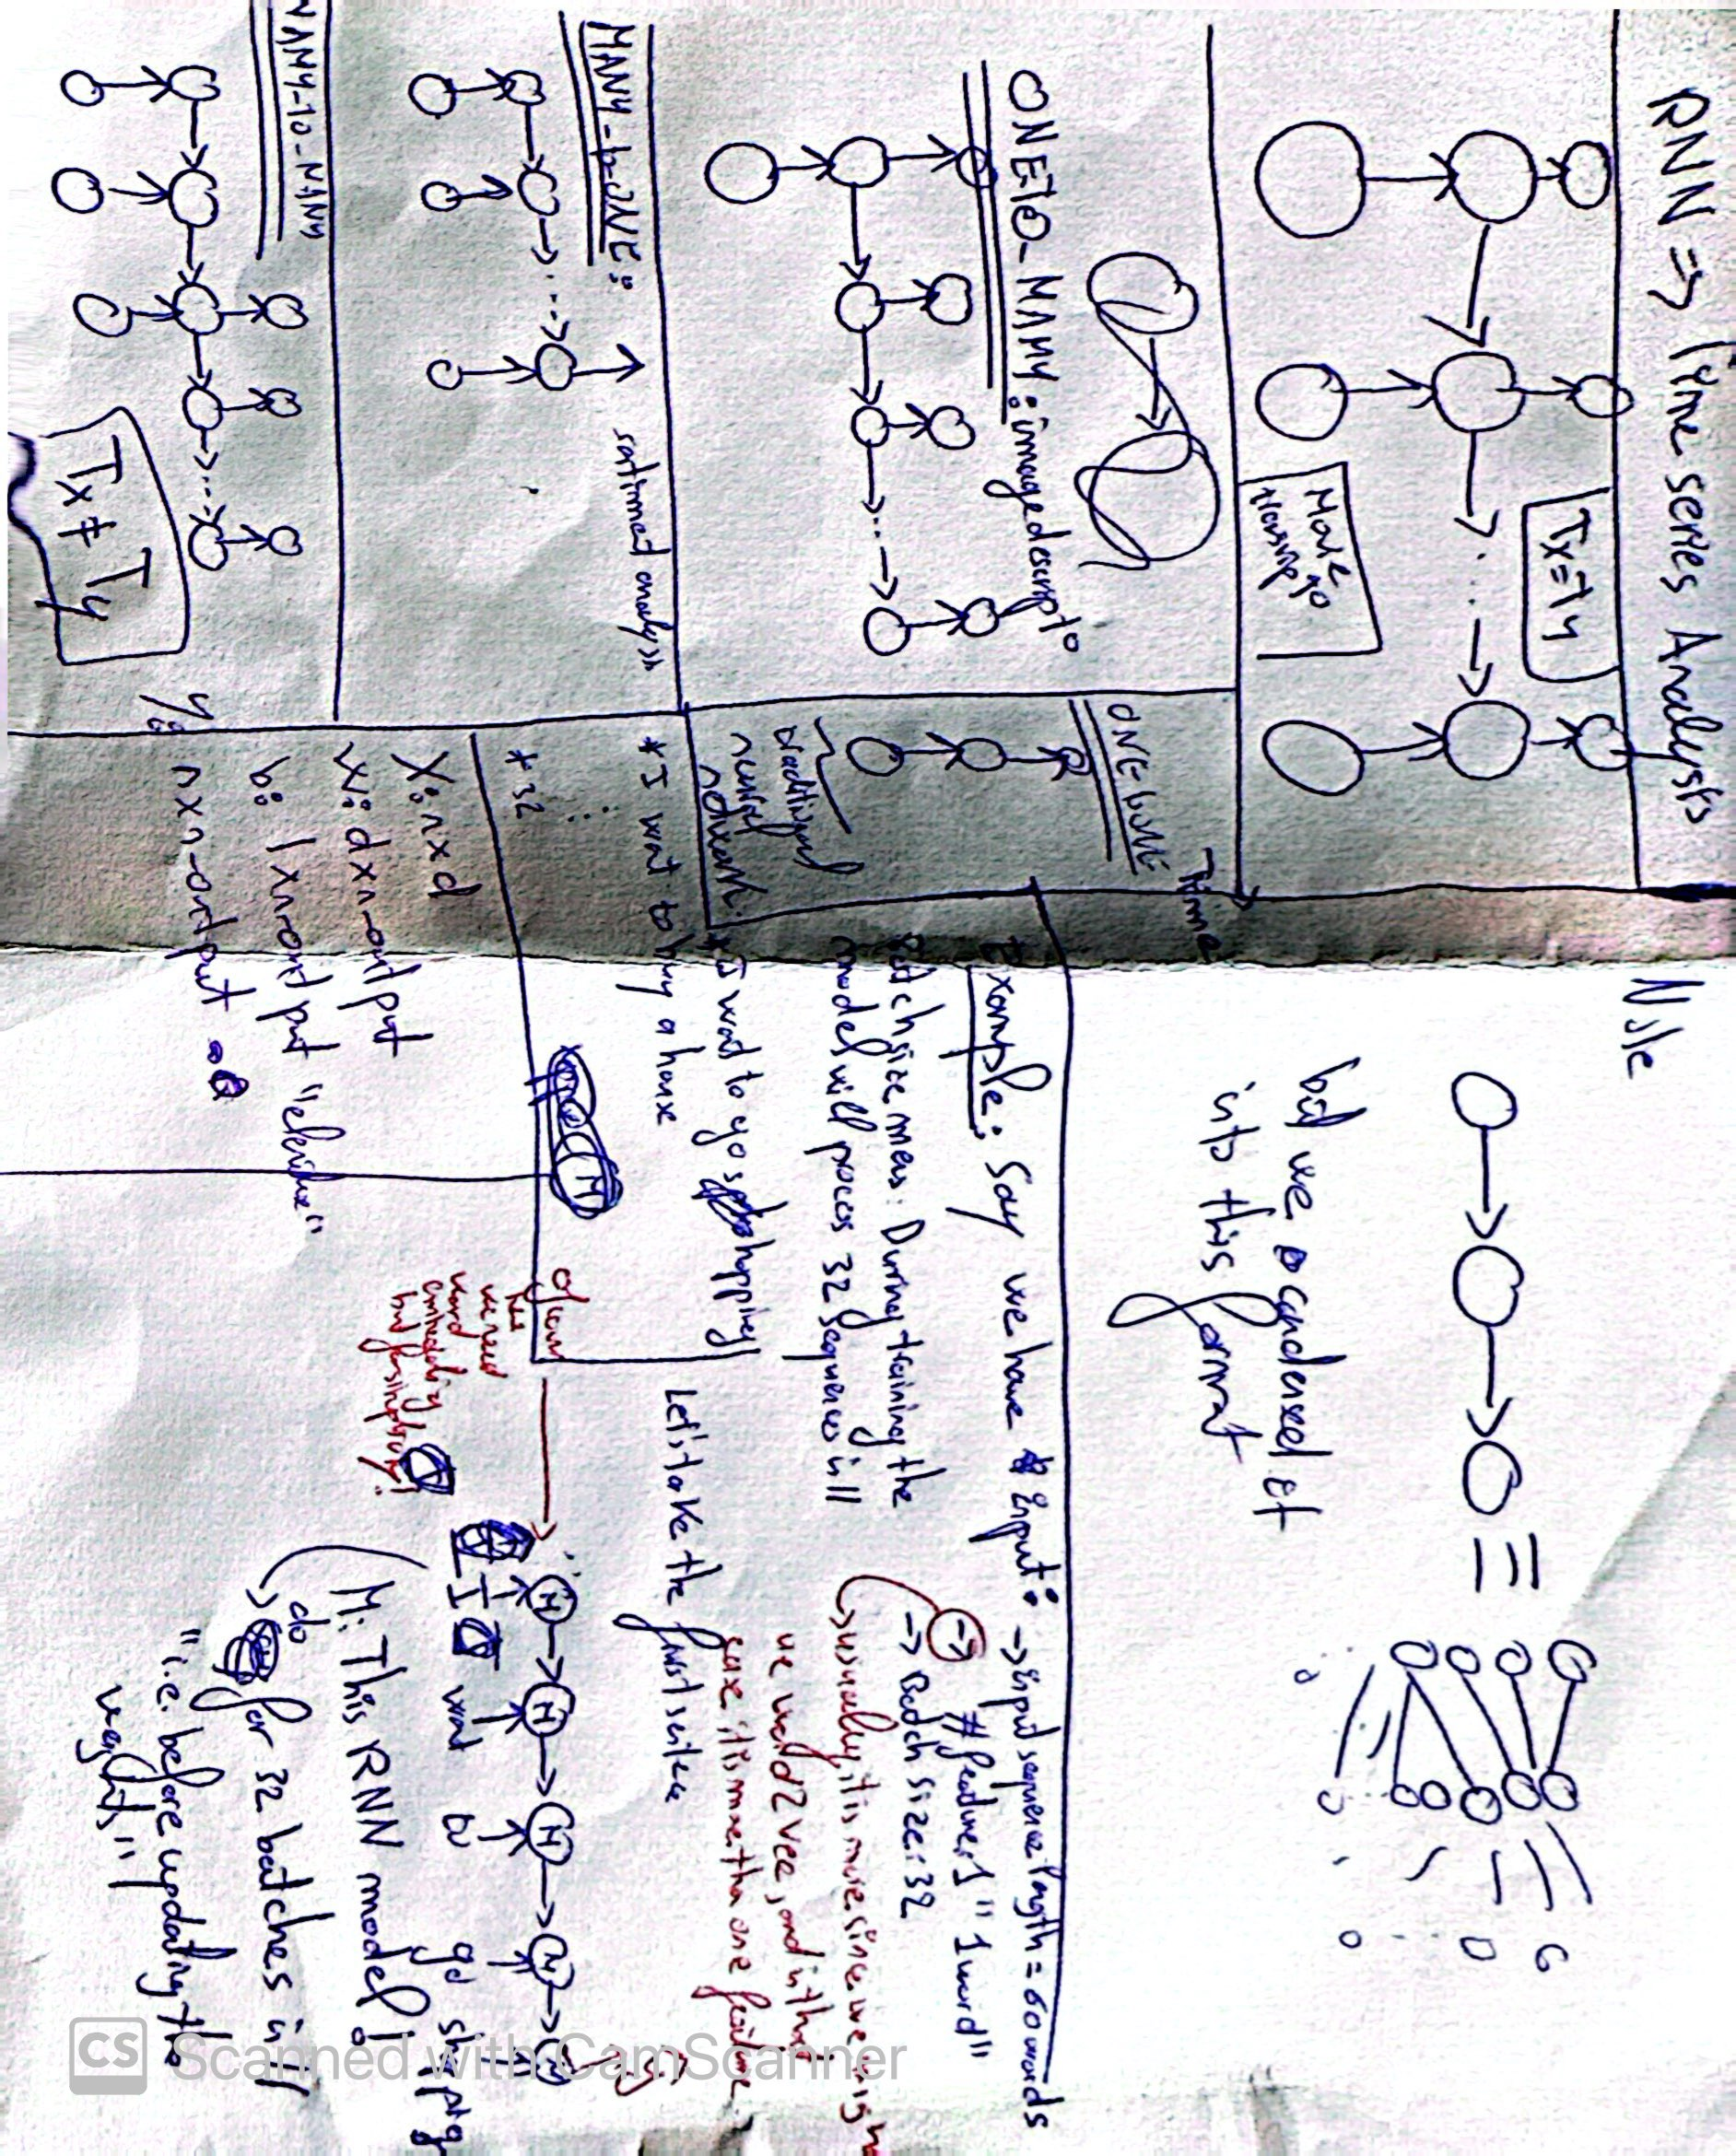
\includegraphics[width = \textwidth]{Images/2_.jpg}
    \caption{Scketch - Helper}
  \end{figure}
  \begin{figure}
    \centering
    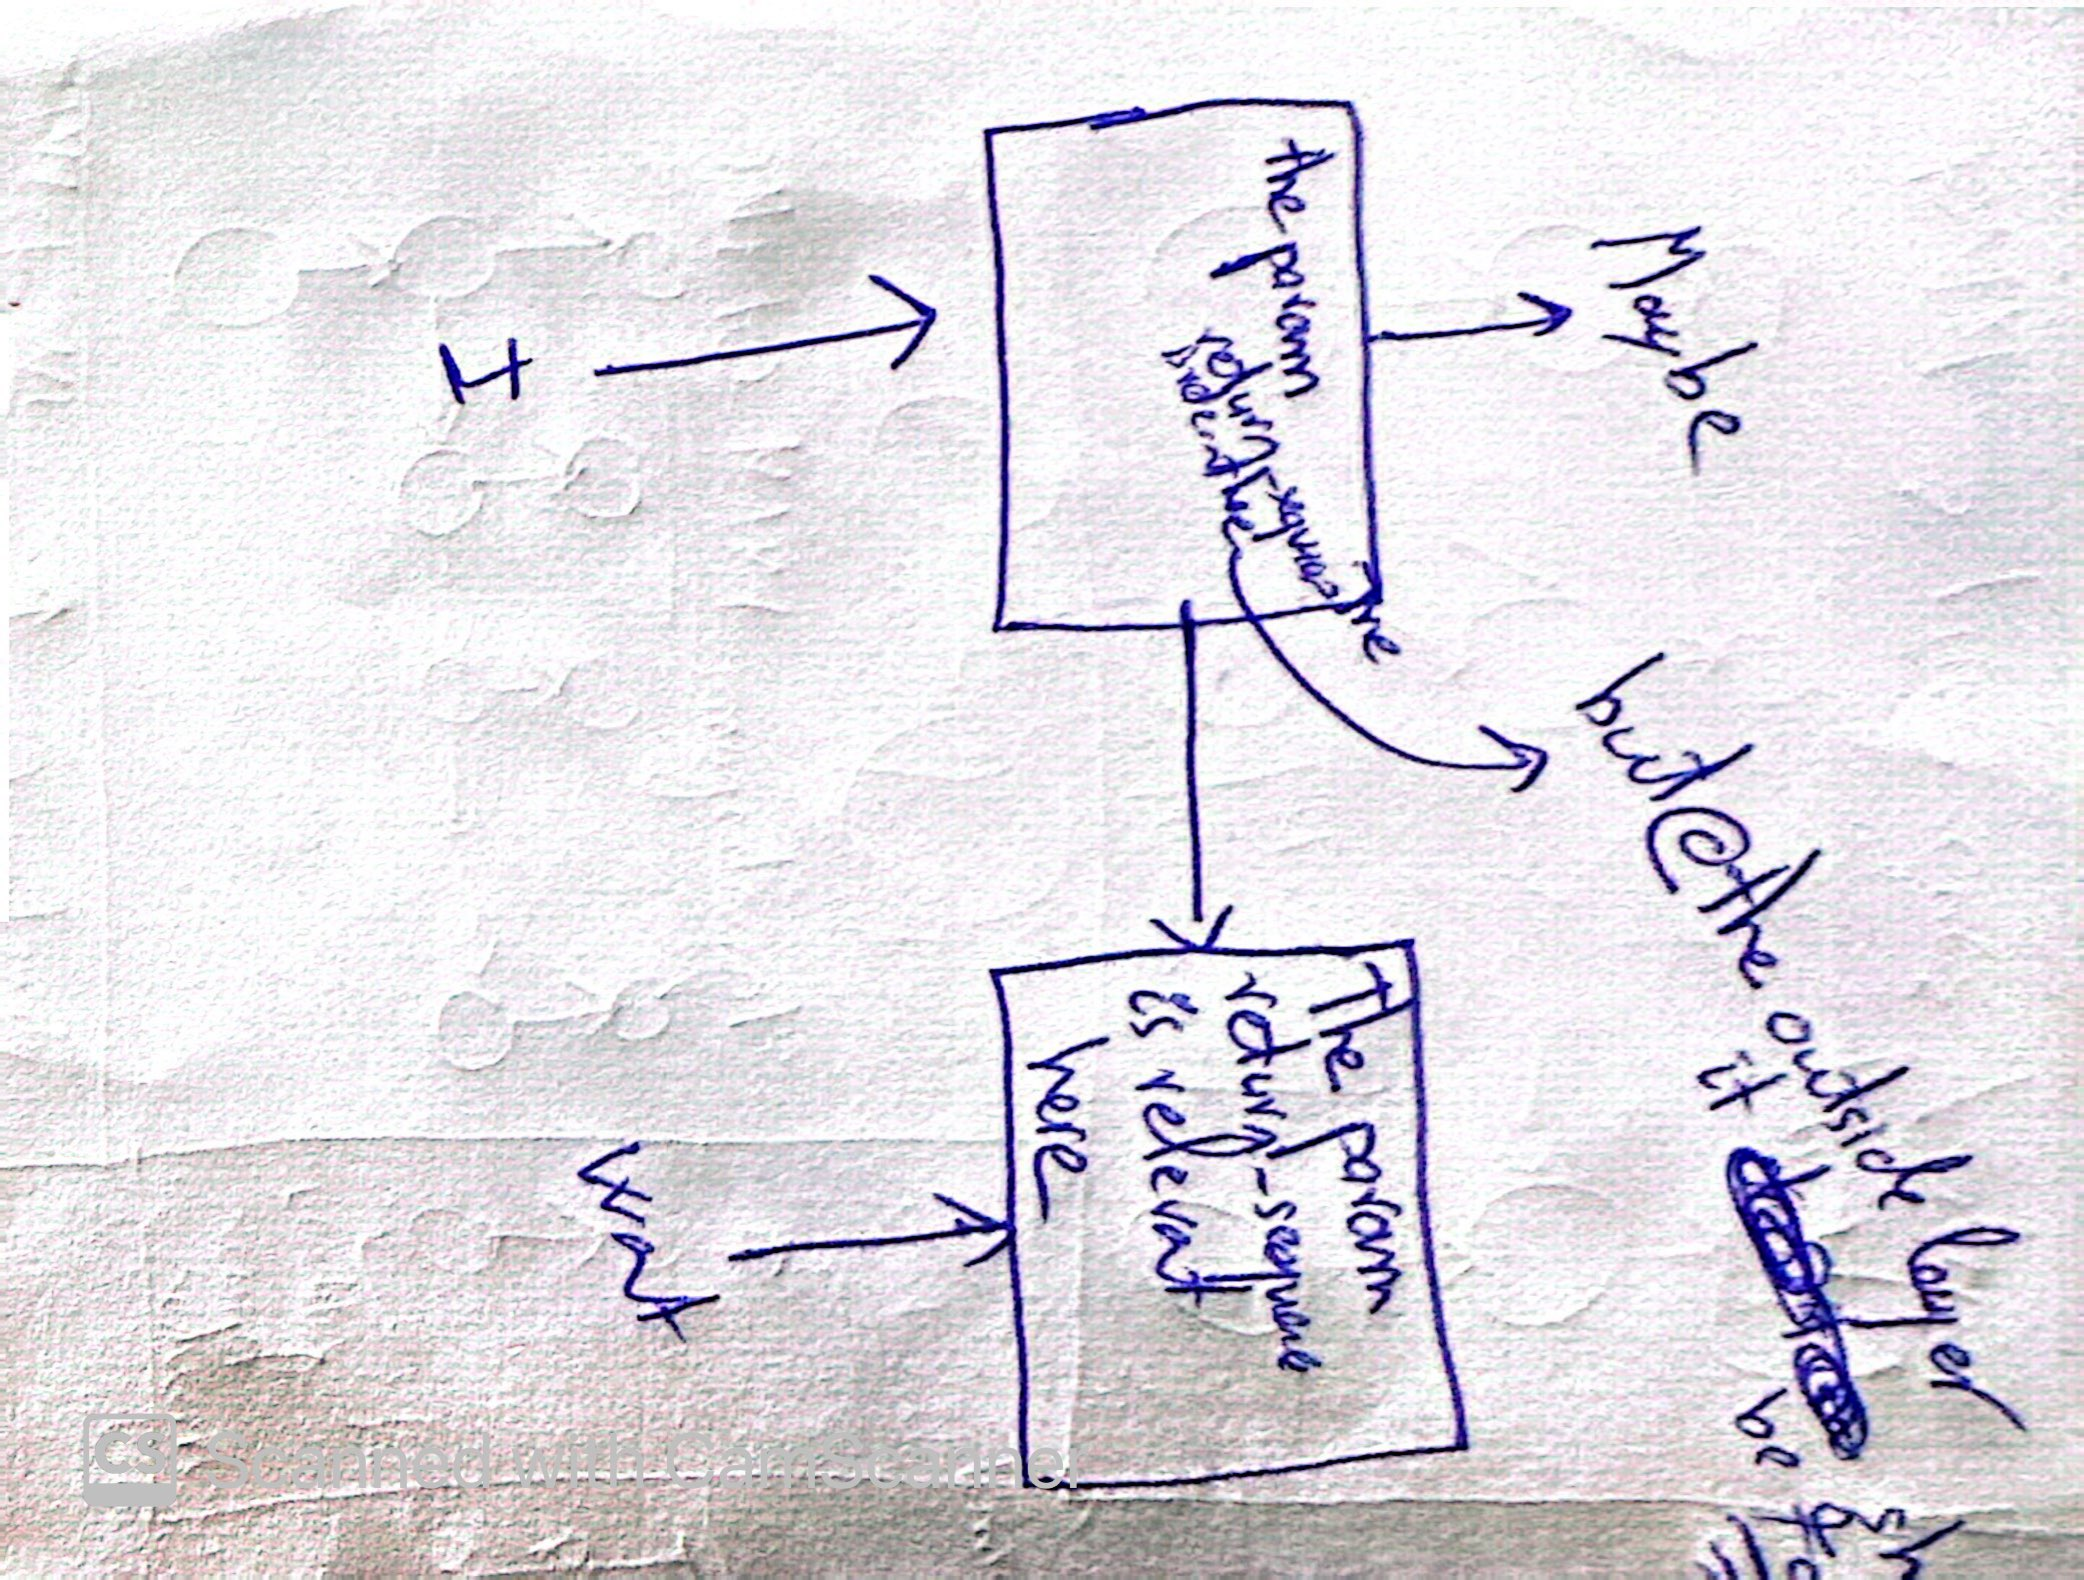
\includegraphics[width = \textwidth]{Images/3_.jpg}
    \caption{Scketch - Helper}
  \end{figure}
  \begin{itemize}
    \item We use Backpropagation through time (BPTT).
    \item But you might see that there is a problem with this, because the gradients might explode or vanish, because of the Long Sequences and Long dependencies.
    \item To solve this we have Many ways to do so:
    \item Proper use of activation functions to solve the gradient vanishing problem: 
    \begin{figure}[H]
      \centering
      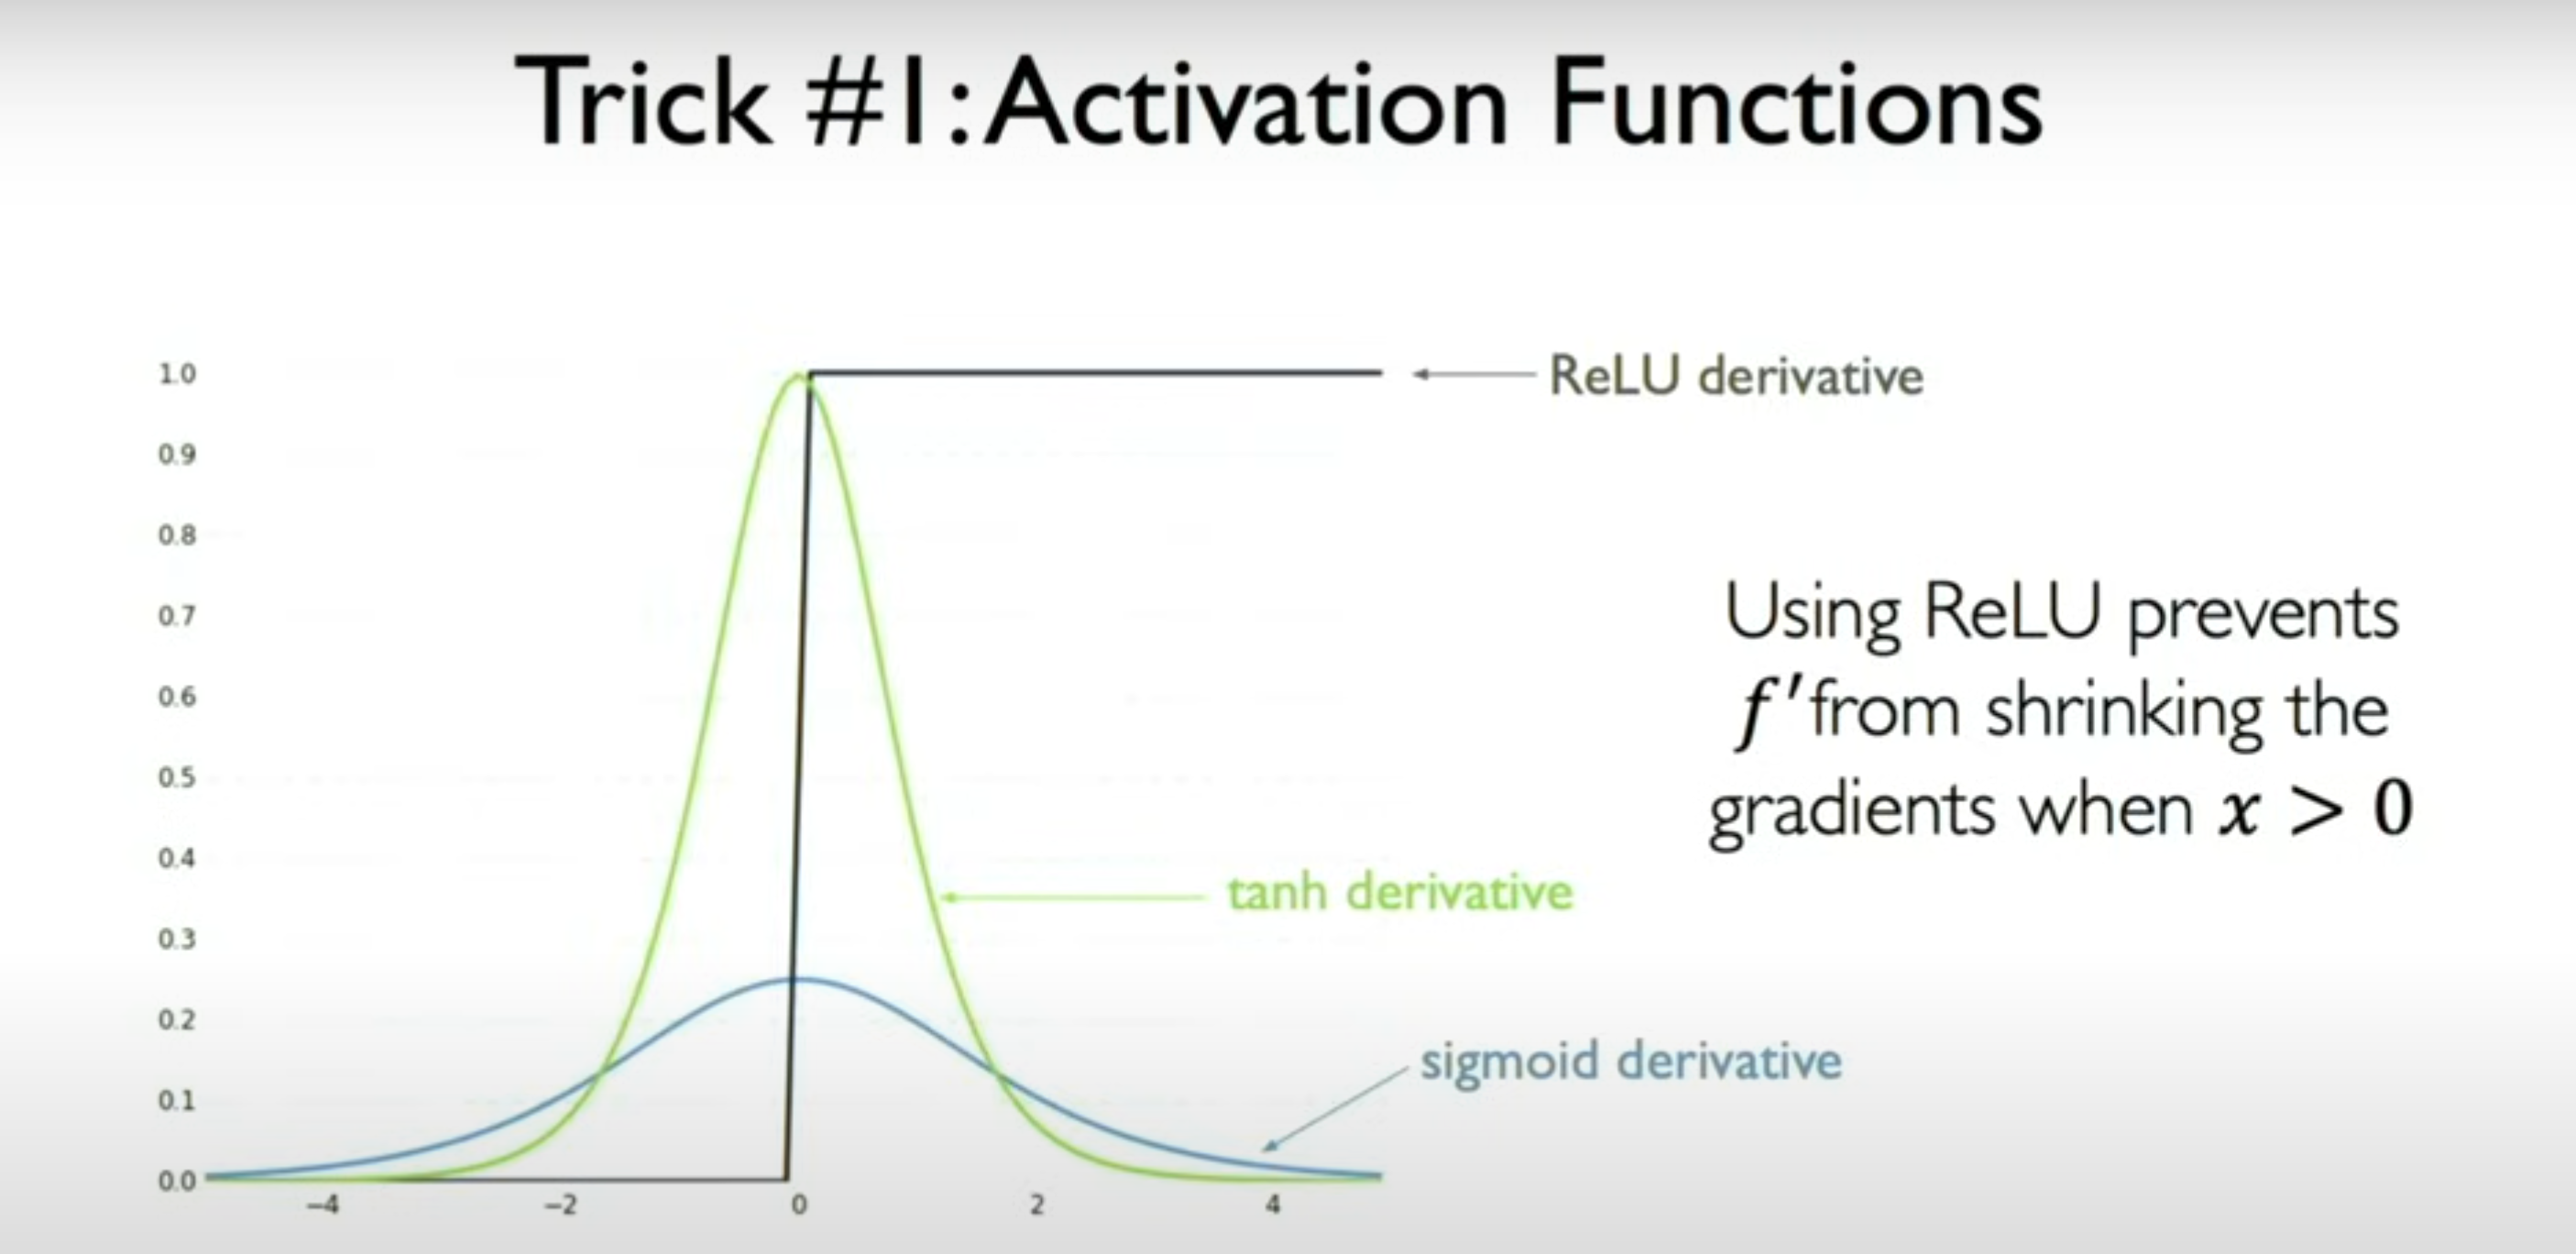
\includegraphics[width = \textwidth]{Images/rnn7.png}
      \caption{ReLU - A Good Choice for Activation Functions}
    \end{figure}
    \item LSTM: Long Short Term Memory, it has a cell state that goes through the sequence, and it has gates that control the flow of information. Meaning that it can decide what to forget and what to remember.(How it decides what to forget and what to remember? It is learned from the data, so it is a learned parameter).
    \item Key Concepts of LSTM: Maintain the cell state, Forget gate, Input gate, Output gate.In the LSTM Backpropagation happens through time with \underline{Partially} uninterrupted gradient flow.
    \begin{figure}[H]
      \centering
      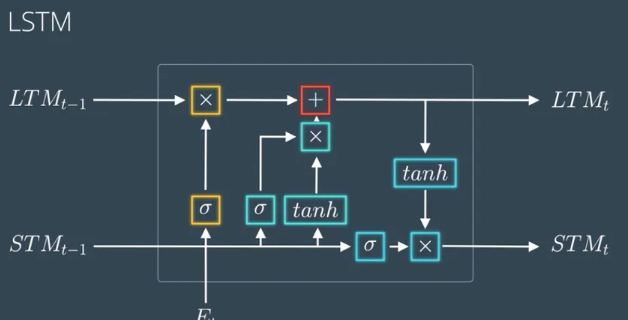
\includegraphics[width = \textwidth]{Images/lstm.png}
      \caption{LSTM}
    \end{figure}
    \item GRU: Gated Recurrent Unit, it is a simplified version of the LSTM, it has a reset gate and an update gate. It is faster to train than the LSTM. 
    \begin{figure}[H]
      \centering
      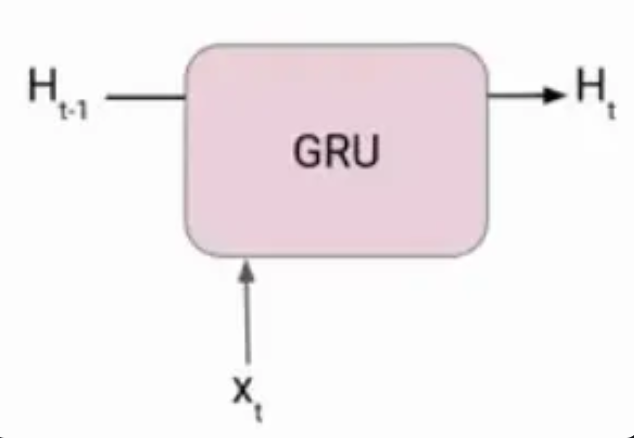
\includegraphics[width = \textwidth]{Images/gru.png}
      \caption{GRU}
    \end{figure}
    \item We can see that ultimately we can see them as a black box that takes an input and gives an output, but each model whether (Basic RNN, LSTM, GRU) has its own architecture. Each model chooses what to pass to the next time step. RNN: Passes everything(you might think that this is a good thing, meaning this way we are gaining all information but that is not the case, because of the gradient vanishing problem), LSTM and GRU: Chooses what to pass based on the gates.
    \item So we can see that even with LSTM and GRU we still have the problem of the vanishing gradient, but it is less severe than the RNN. So what is the solution? 
  \end{itemize}


  \subsubsection*{\underline{Transformers and Attention Mechanism}}
  \begin{itemize}
    \item Intuition is to build a neural network that will choose what is an important part of the sequence and what is not, so it will focus on the important parts of the sequence. 
    \item What we will focus on is self-attention, so we will focus on the important parts of the sequence
    \item Intuition behind Self-Attention: Identify which parts to attend to, Step 2 Extract the features with high attention 
    \item So in self-attention, we first take the input as a whole (removing the recursion). But we need to make sure we still keep information about the order, how do we do this? We use positional encoding. 
    \begin{figure}[H]
      \centering
      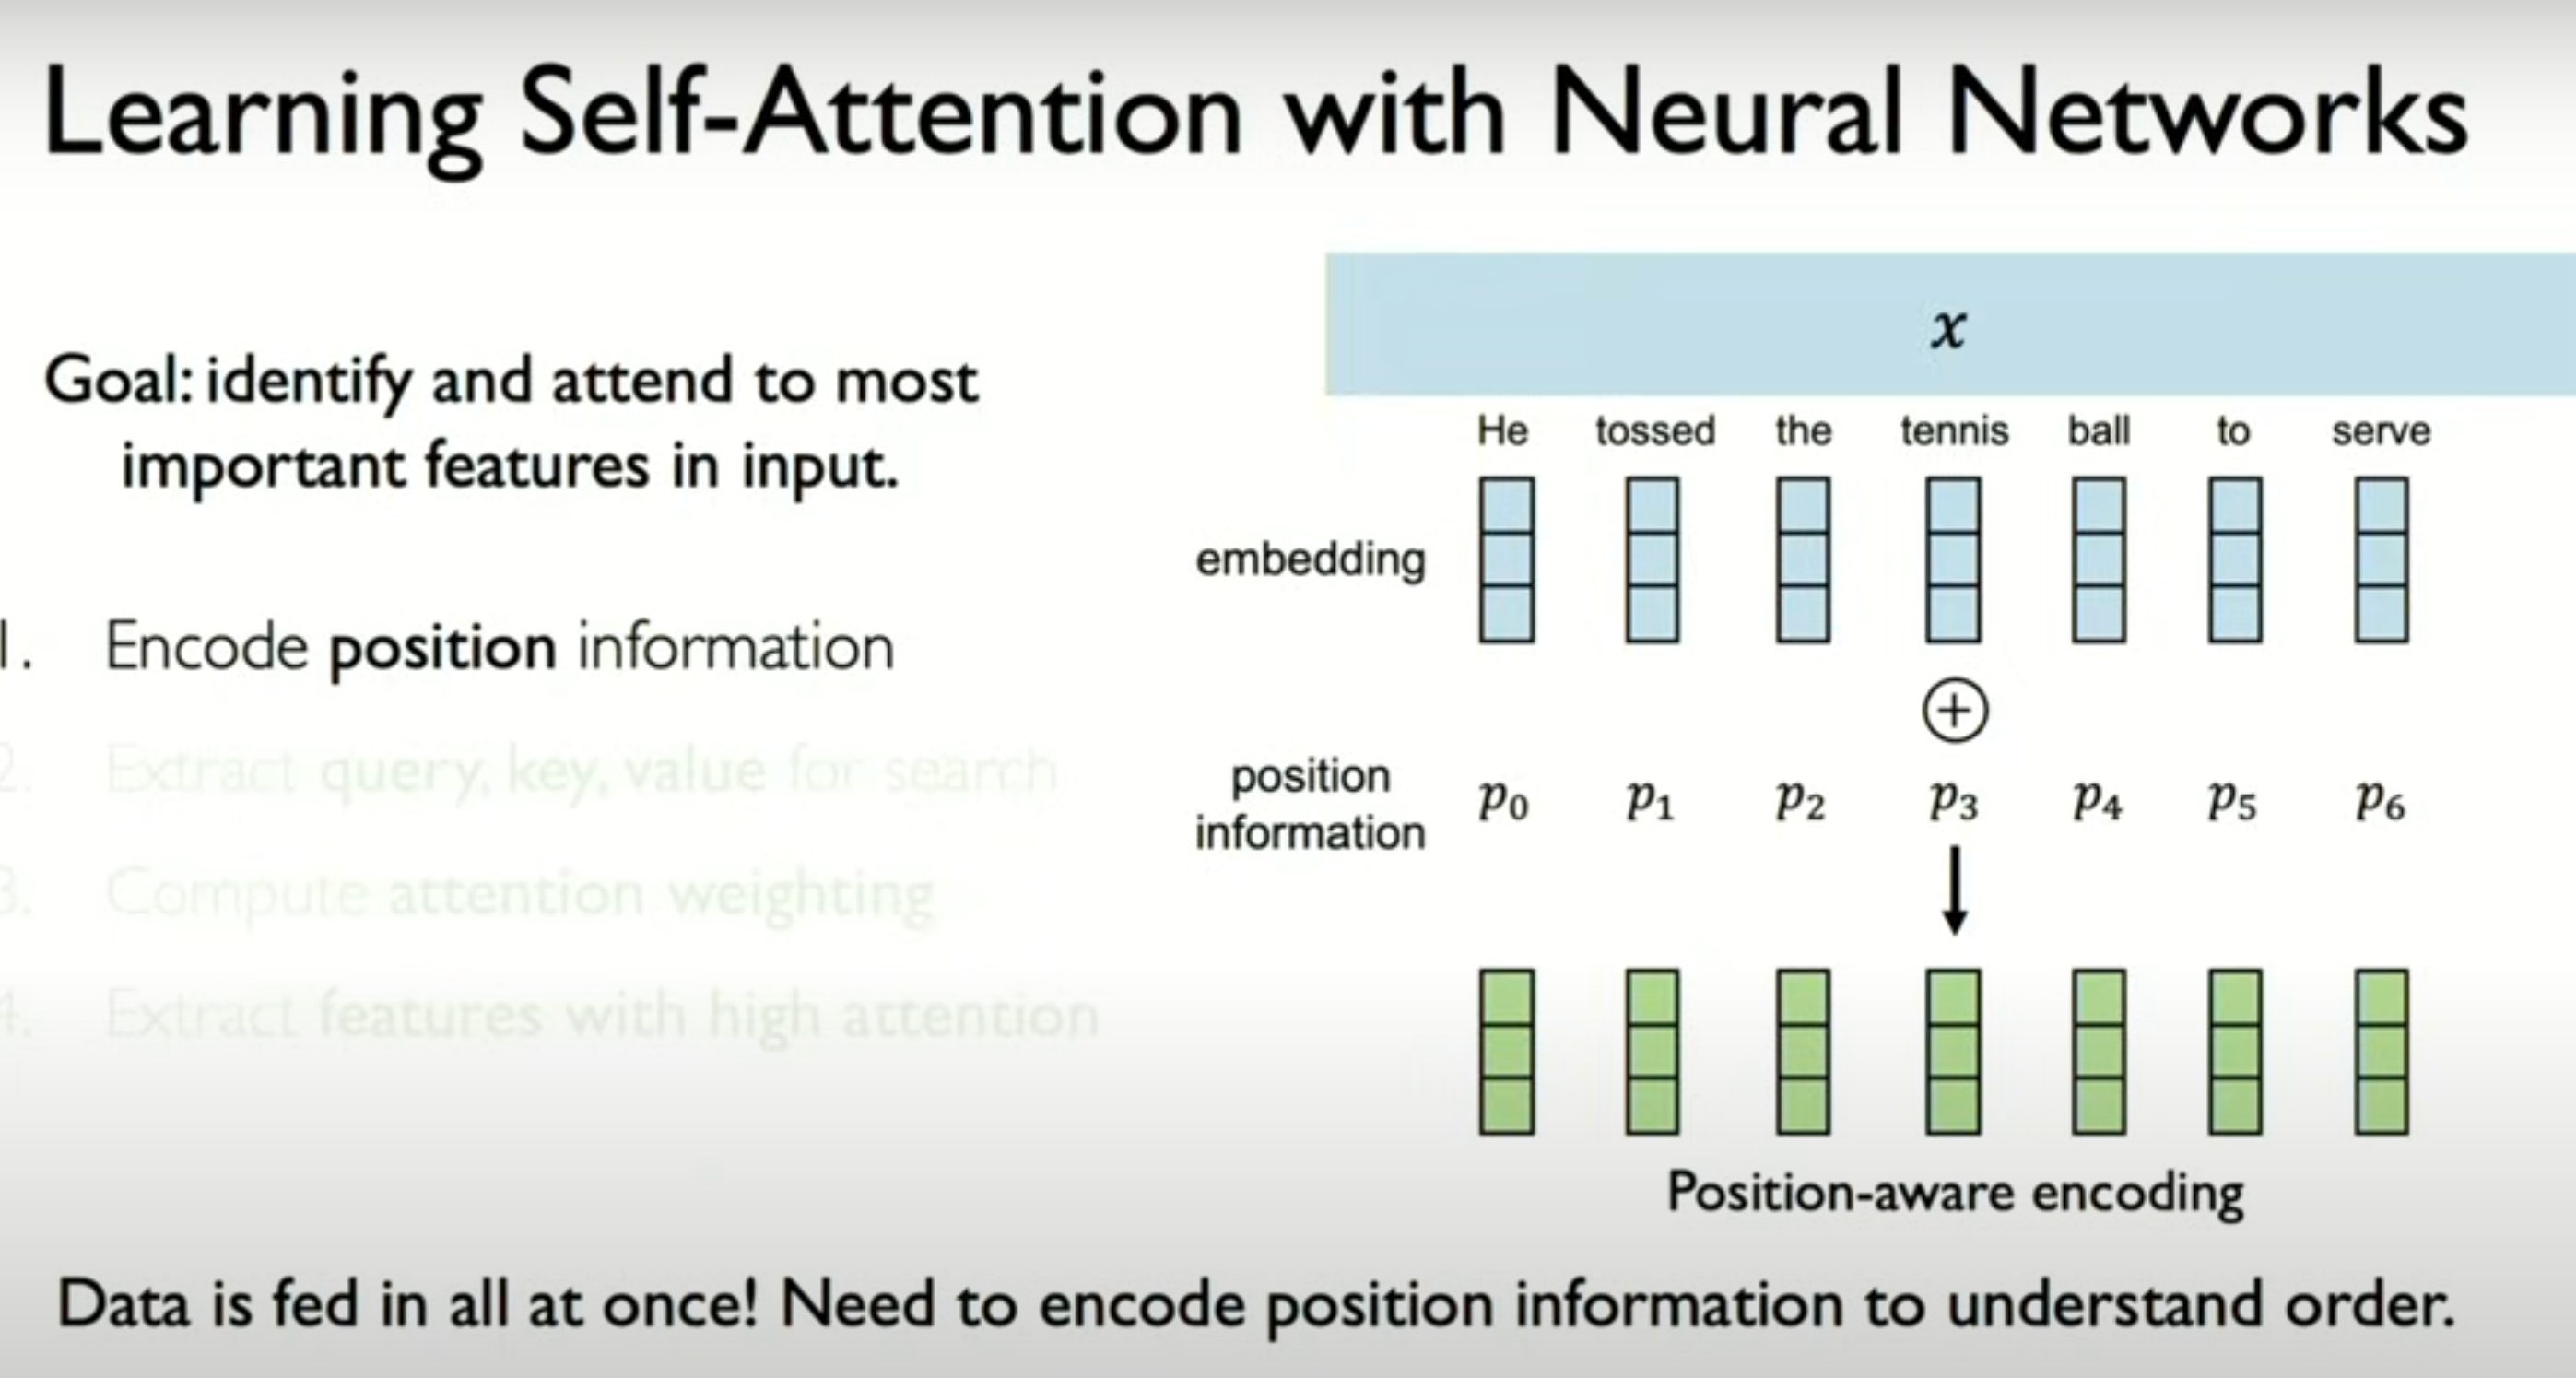
\includegraphics[width = \textwidth]{Images/pae.png}
      \caption{Position-aware Embeddings}
    \end{figure}
    \item Notice that we took the input all at once, we then used our regular word-embedding, then we use position information to keep the order of the sequence to finally get the Position-aware Encoding. So in this way our final embeddings contain information about the order.
    \item Now we need a way to extract query, key, and value from the input. 
    \begin{figure}
      \centering
      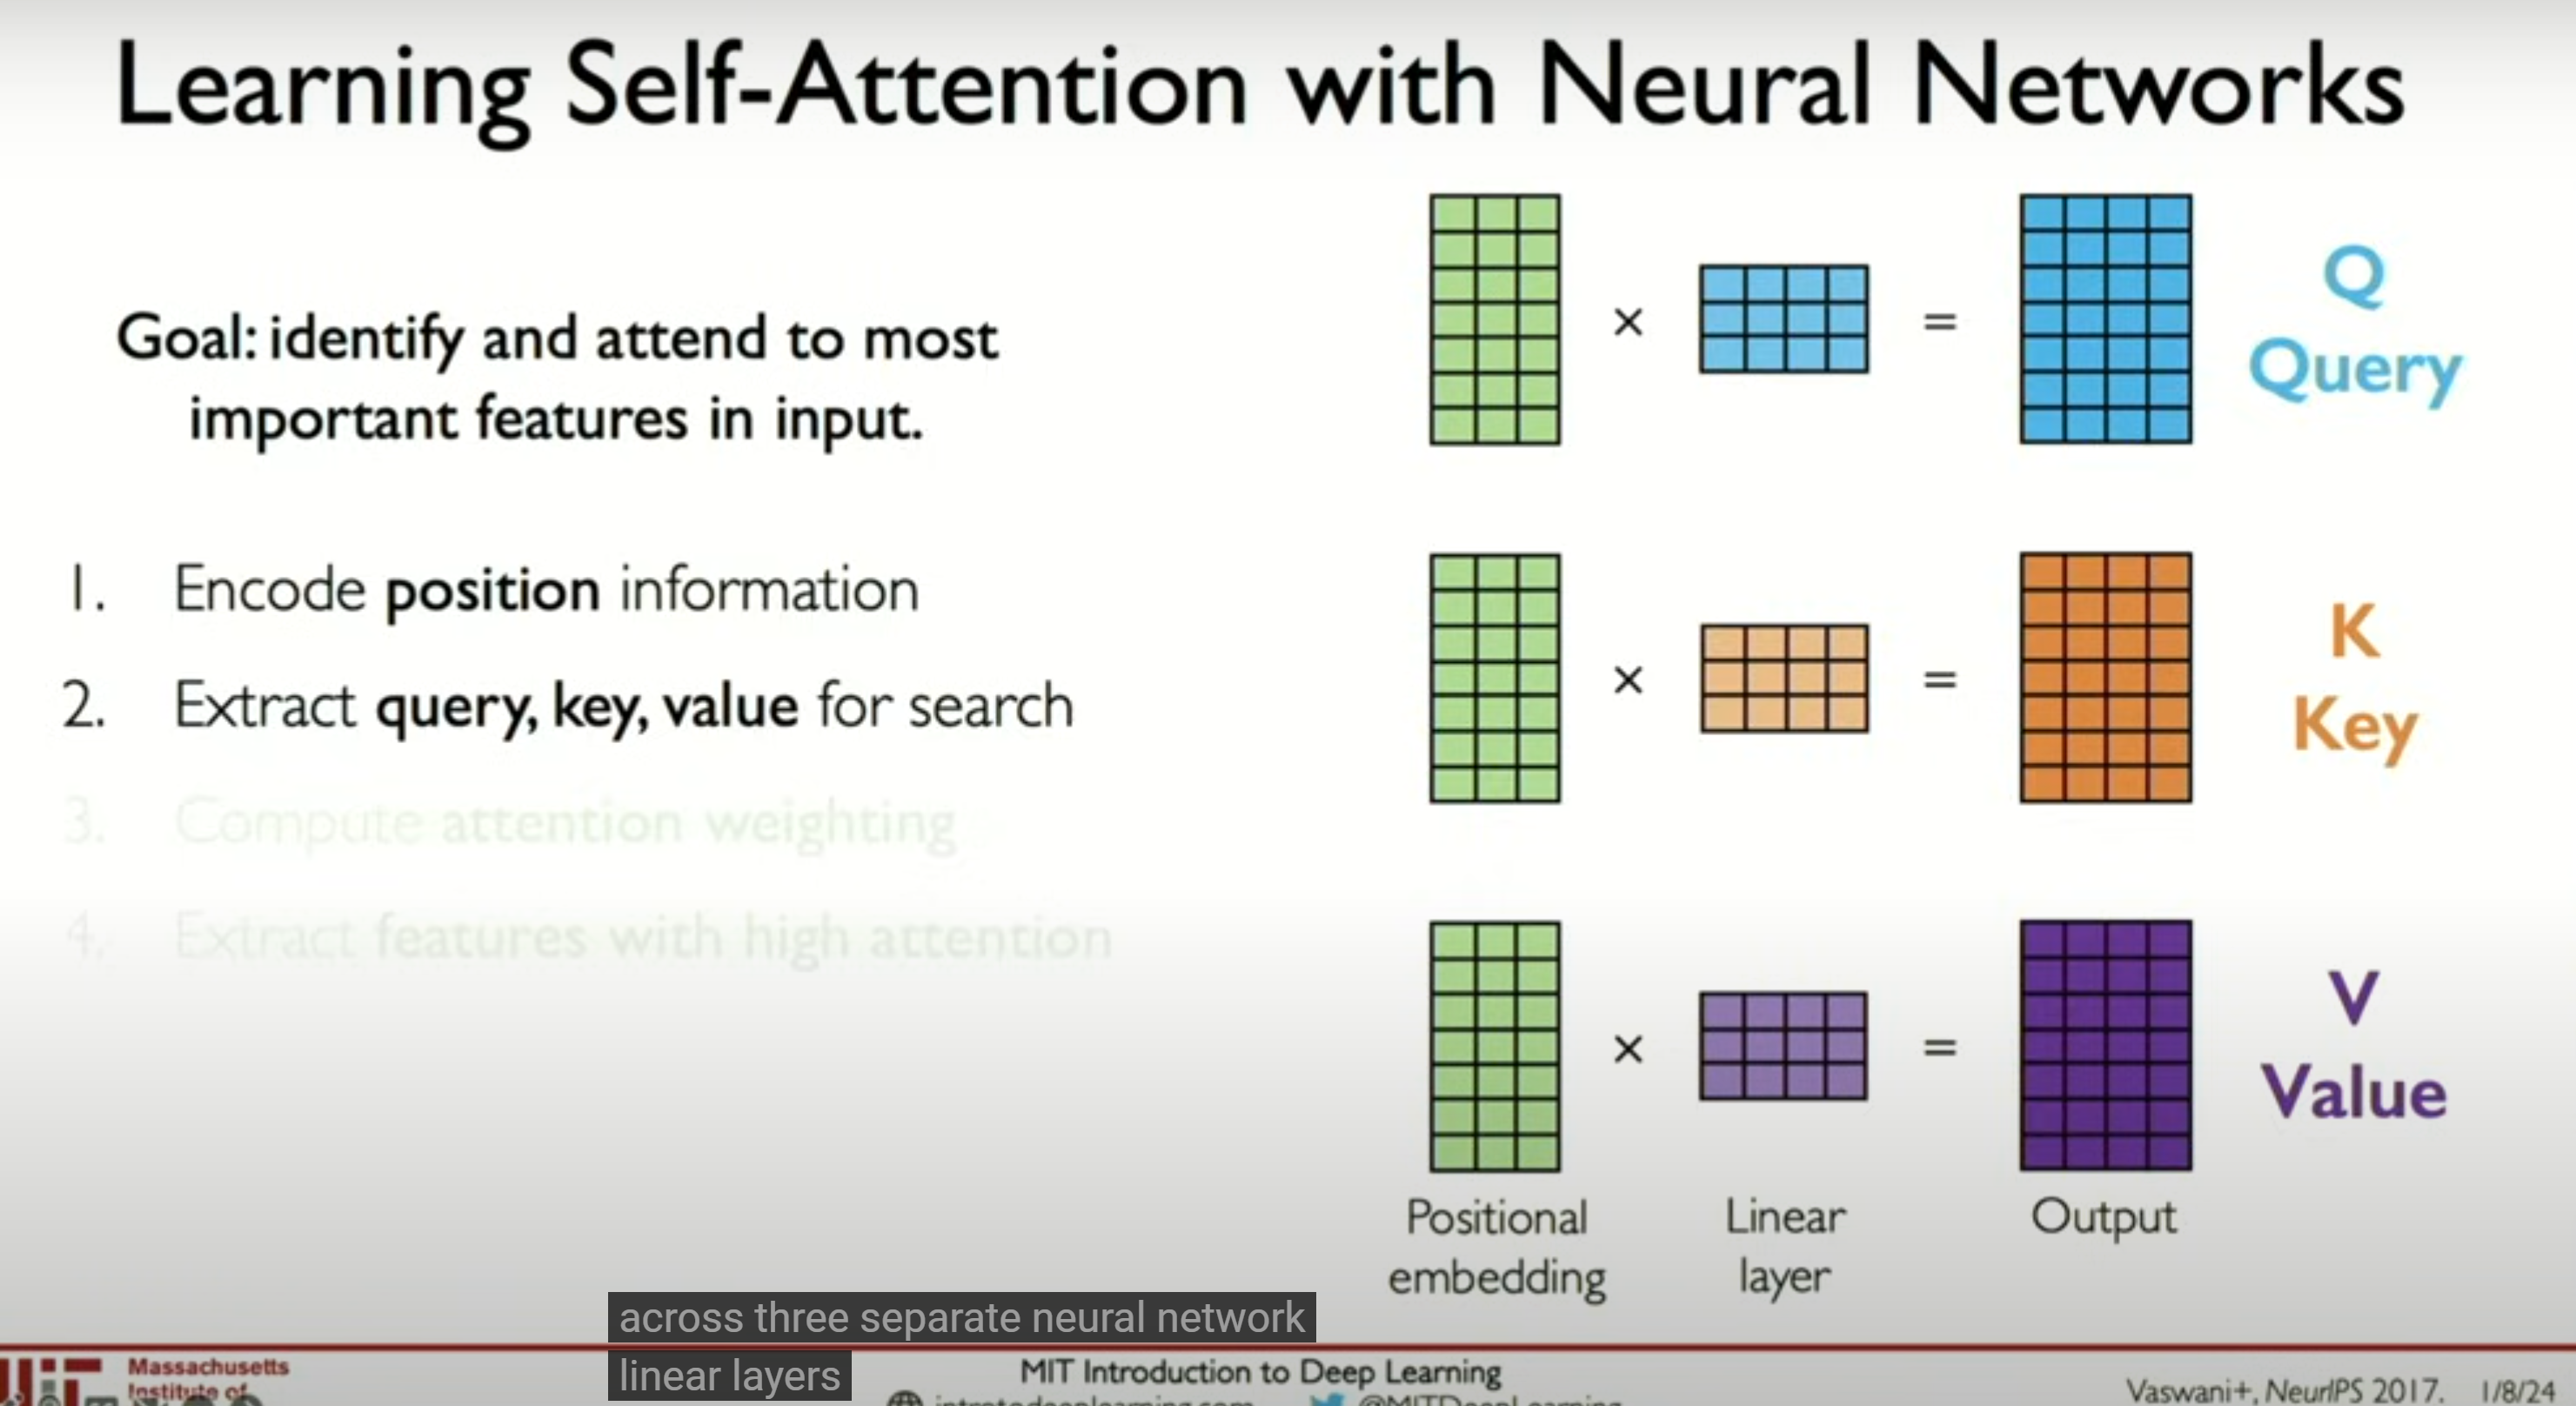
\includegraphics[width = \textwidth]{Images/qkv.png}
      \caption{Query, Key, Value}
    \end{figure}
    \item So what we do is that we take the PAE and we triplicate it, and then feed each one of them to a separate Linear neural network to get the  Query, Key, and Value. 
    \item Now how do we compute the attention score? We need a way to compute the attention weighting for each word in the sequence. 
    \item To do so we need to compute the pairwise similarity between the query and the key. To do so we use the dot product (also known as cosine similarity). 
    \begin{figure}[H]
      \centering
      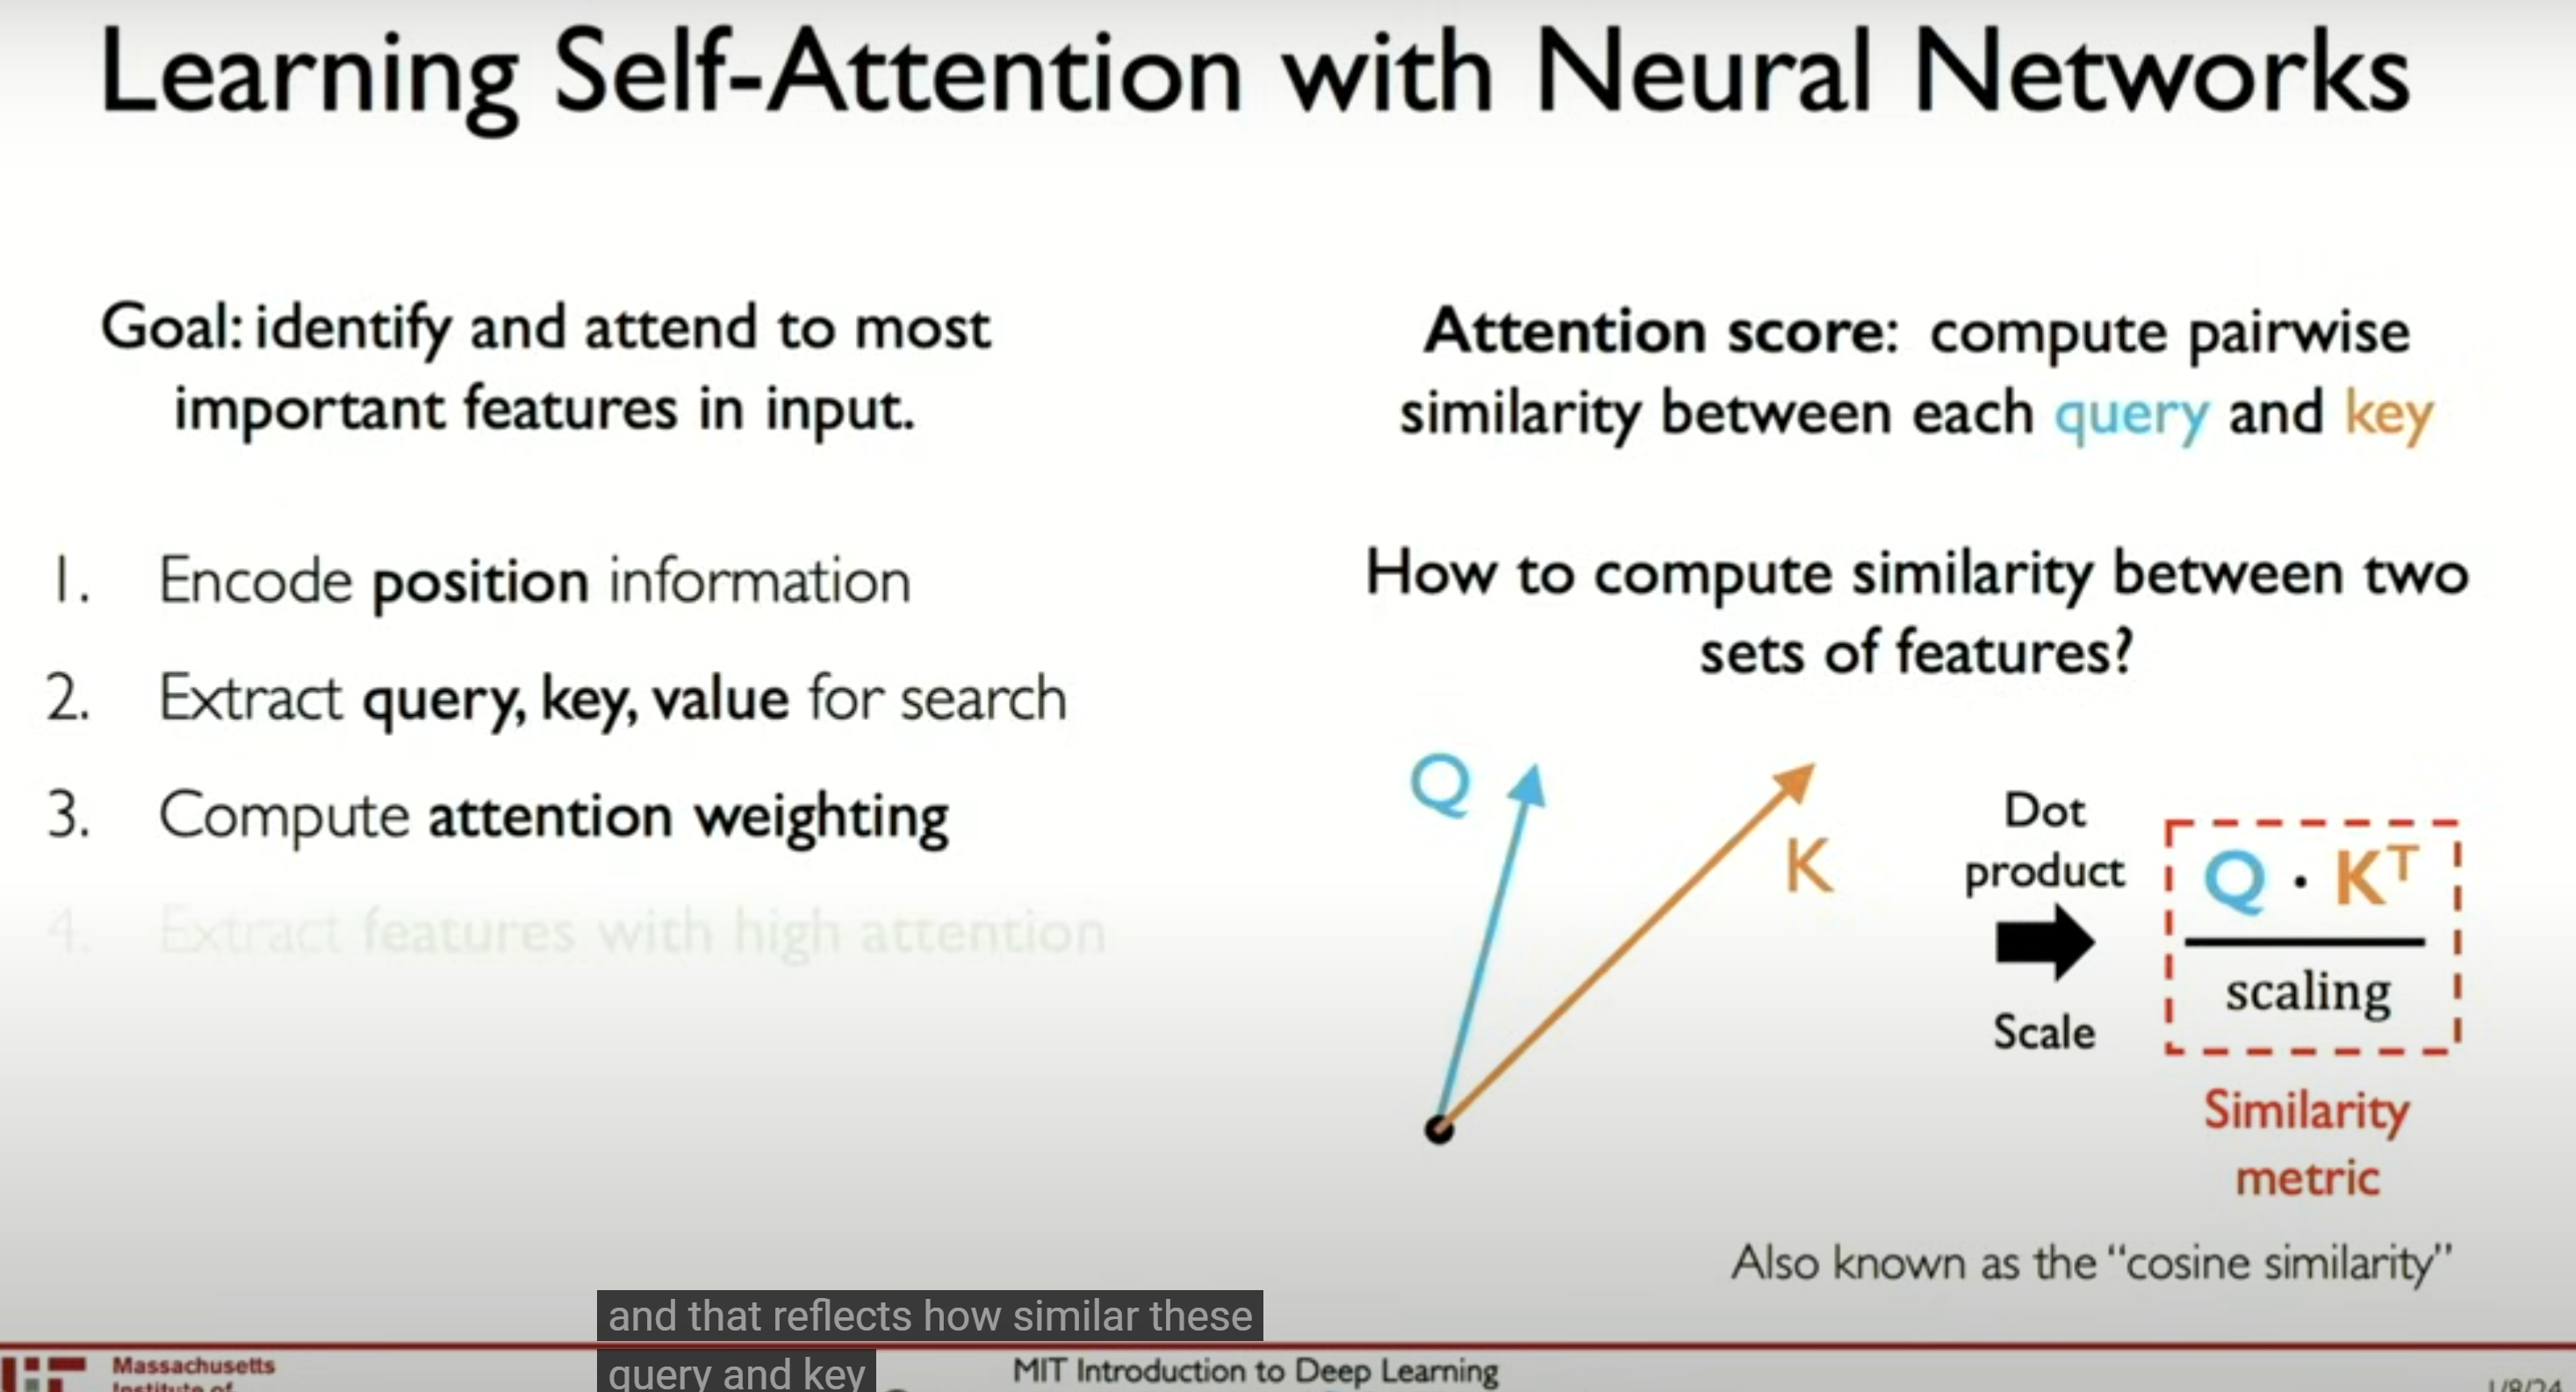
\includegraphics[width = 0.5\textwidth]{Images/attention_score.png}
      \caption{Attention Score}
    \end{figure}
    \item Now we have how similar each word is to the query, but we need to normalize this, so we use the softmax function. 
    
    \begin{figure}[H]
      \centering
      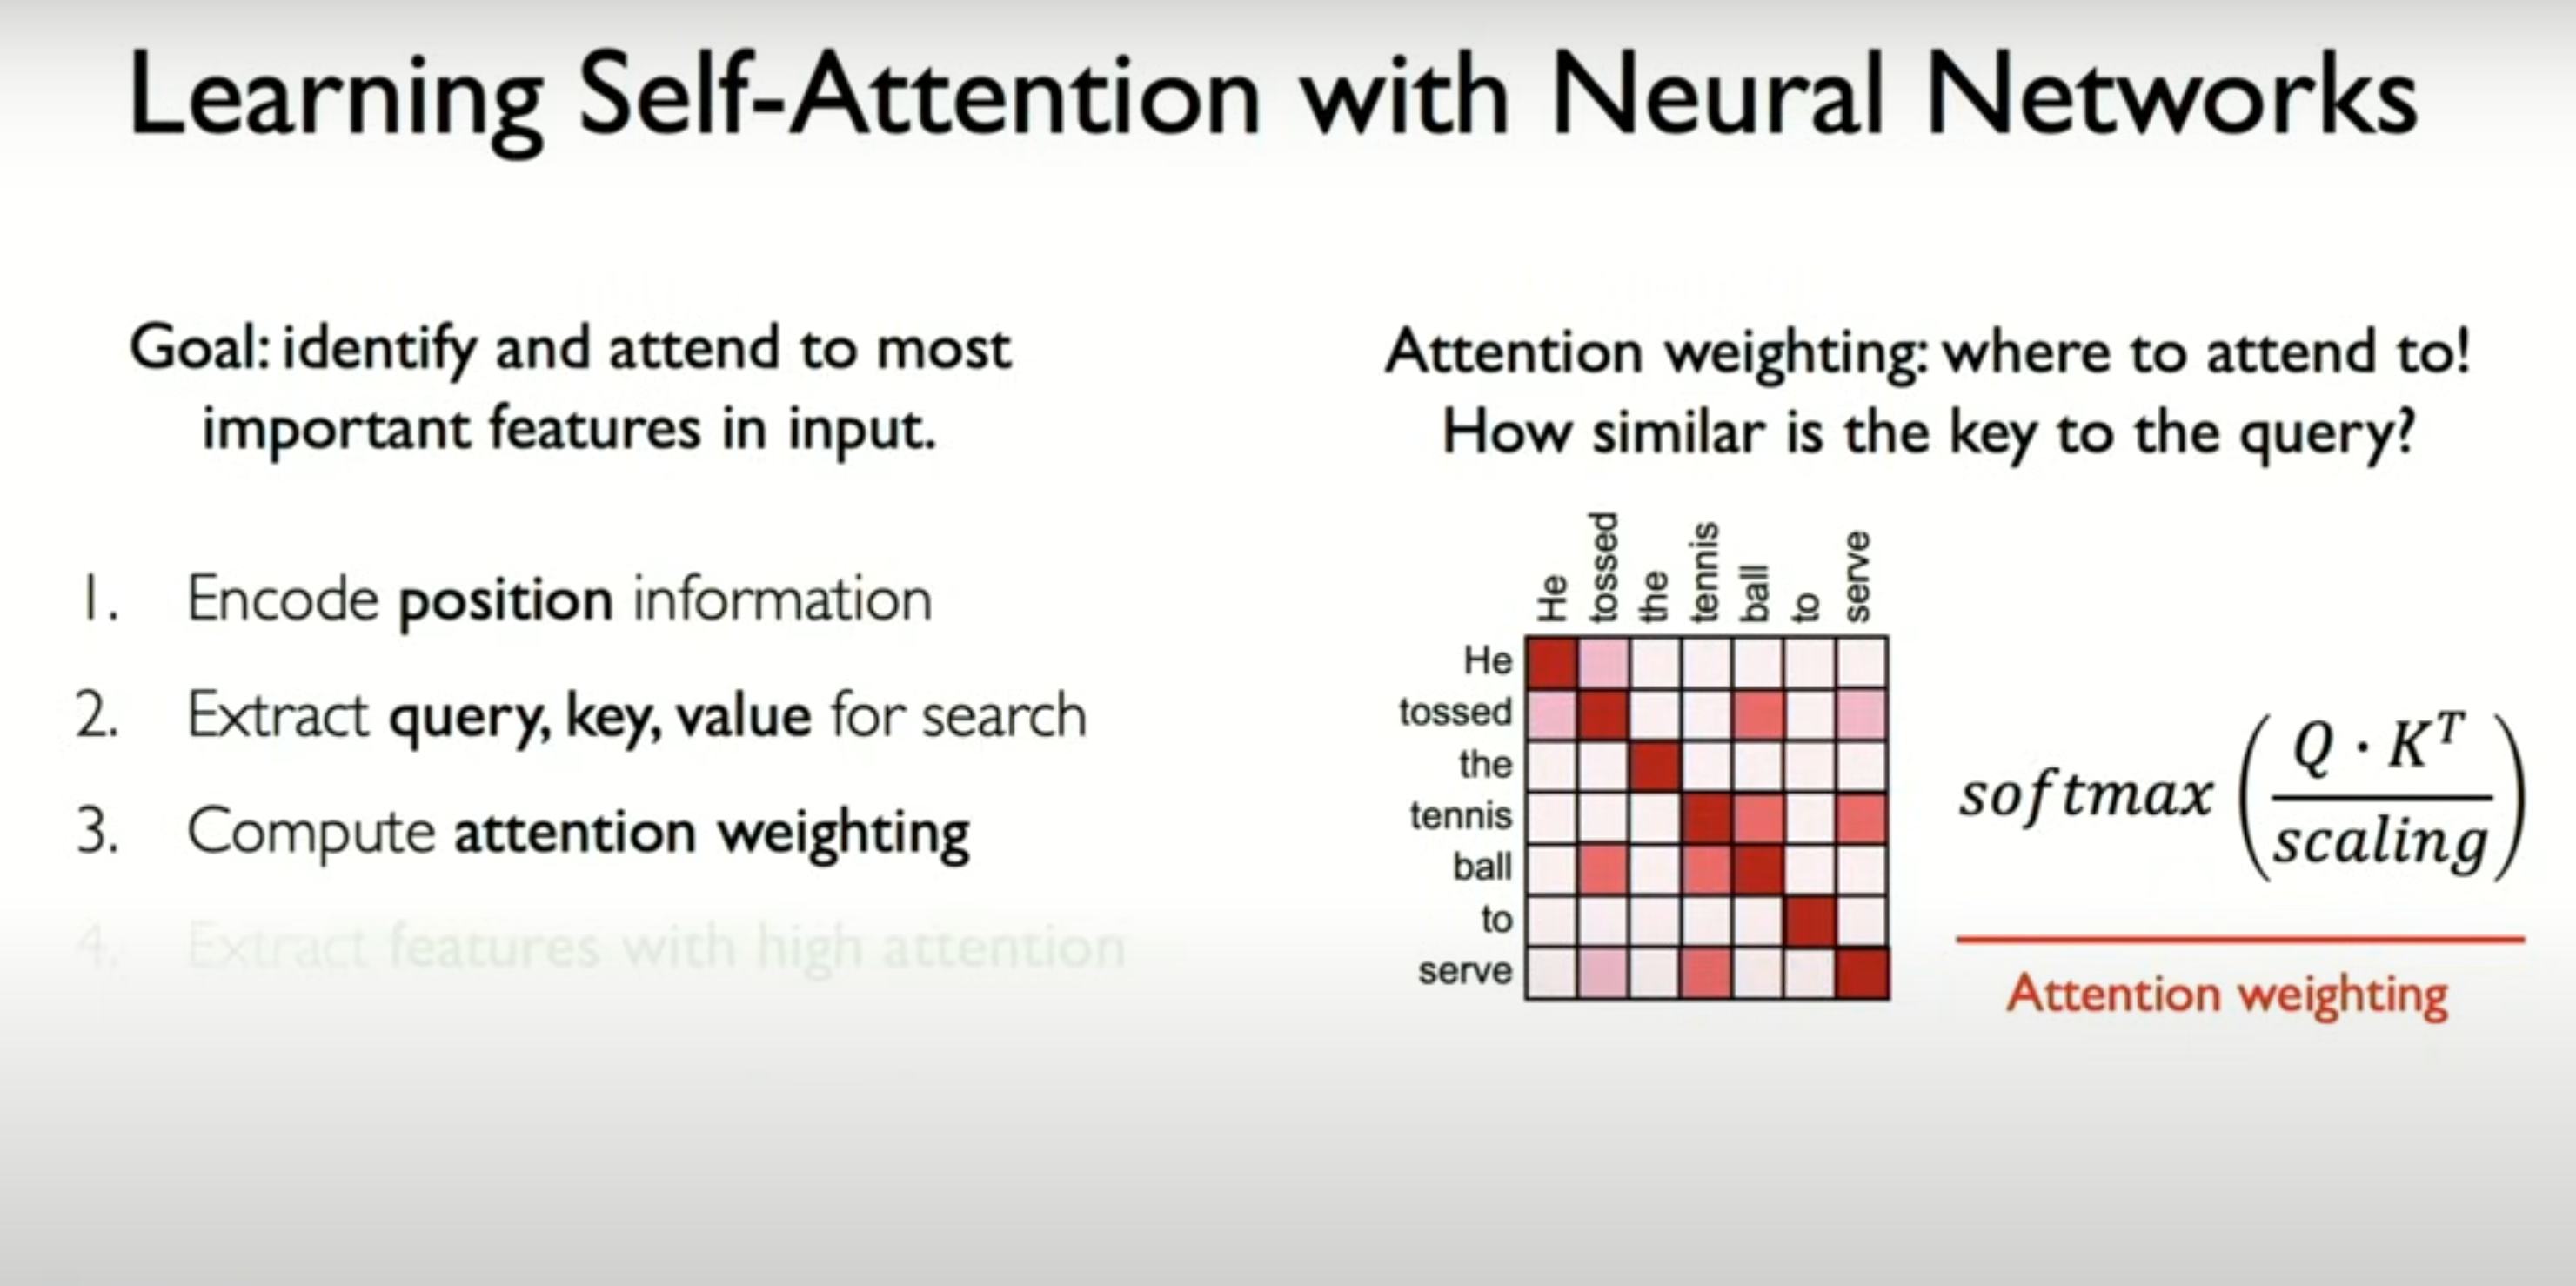
\includegraphics[width = 0.5\textwidth]{Images/attention_score2.png}
      \caption{Attention Score - Normalized}
    \end{figure}
    \item Remember that our goal is to extract the most important features in the input based on the highest attention score.
    \begin{figure}[H]
      \centering
      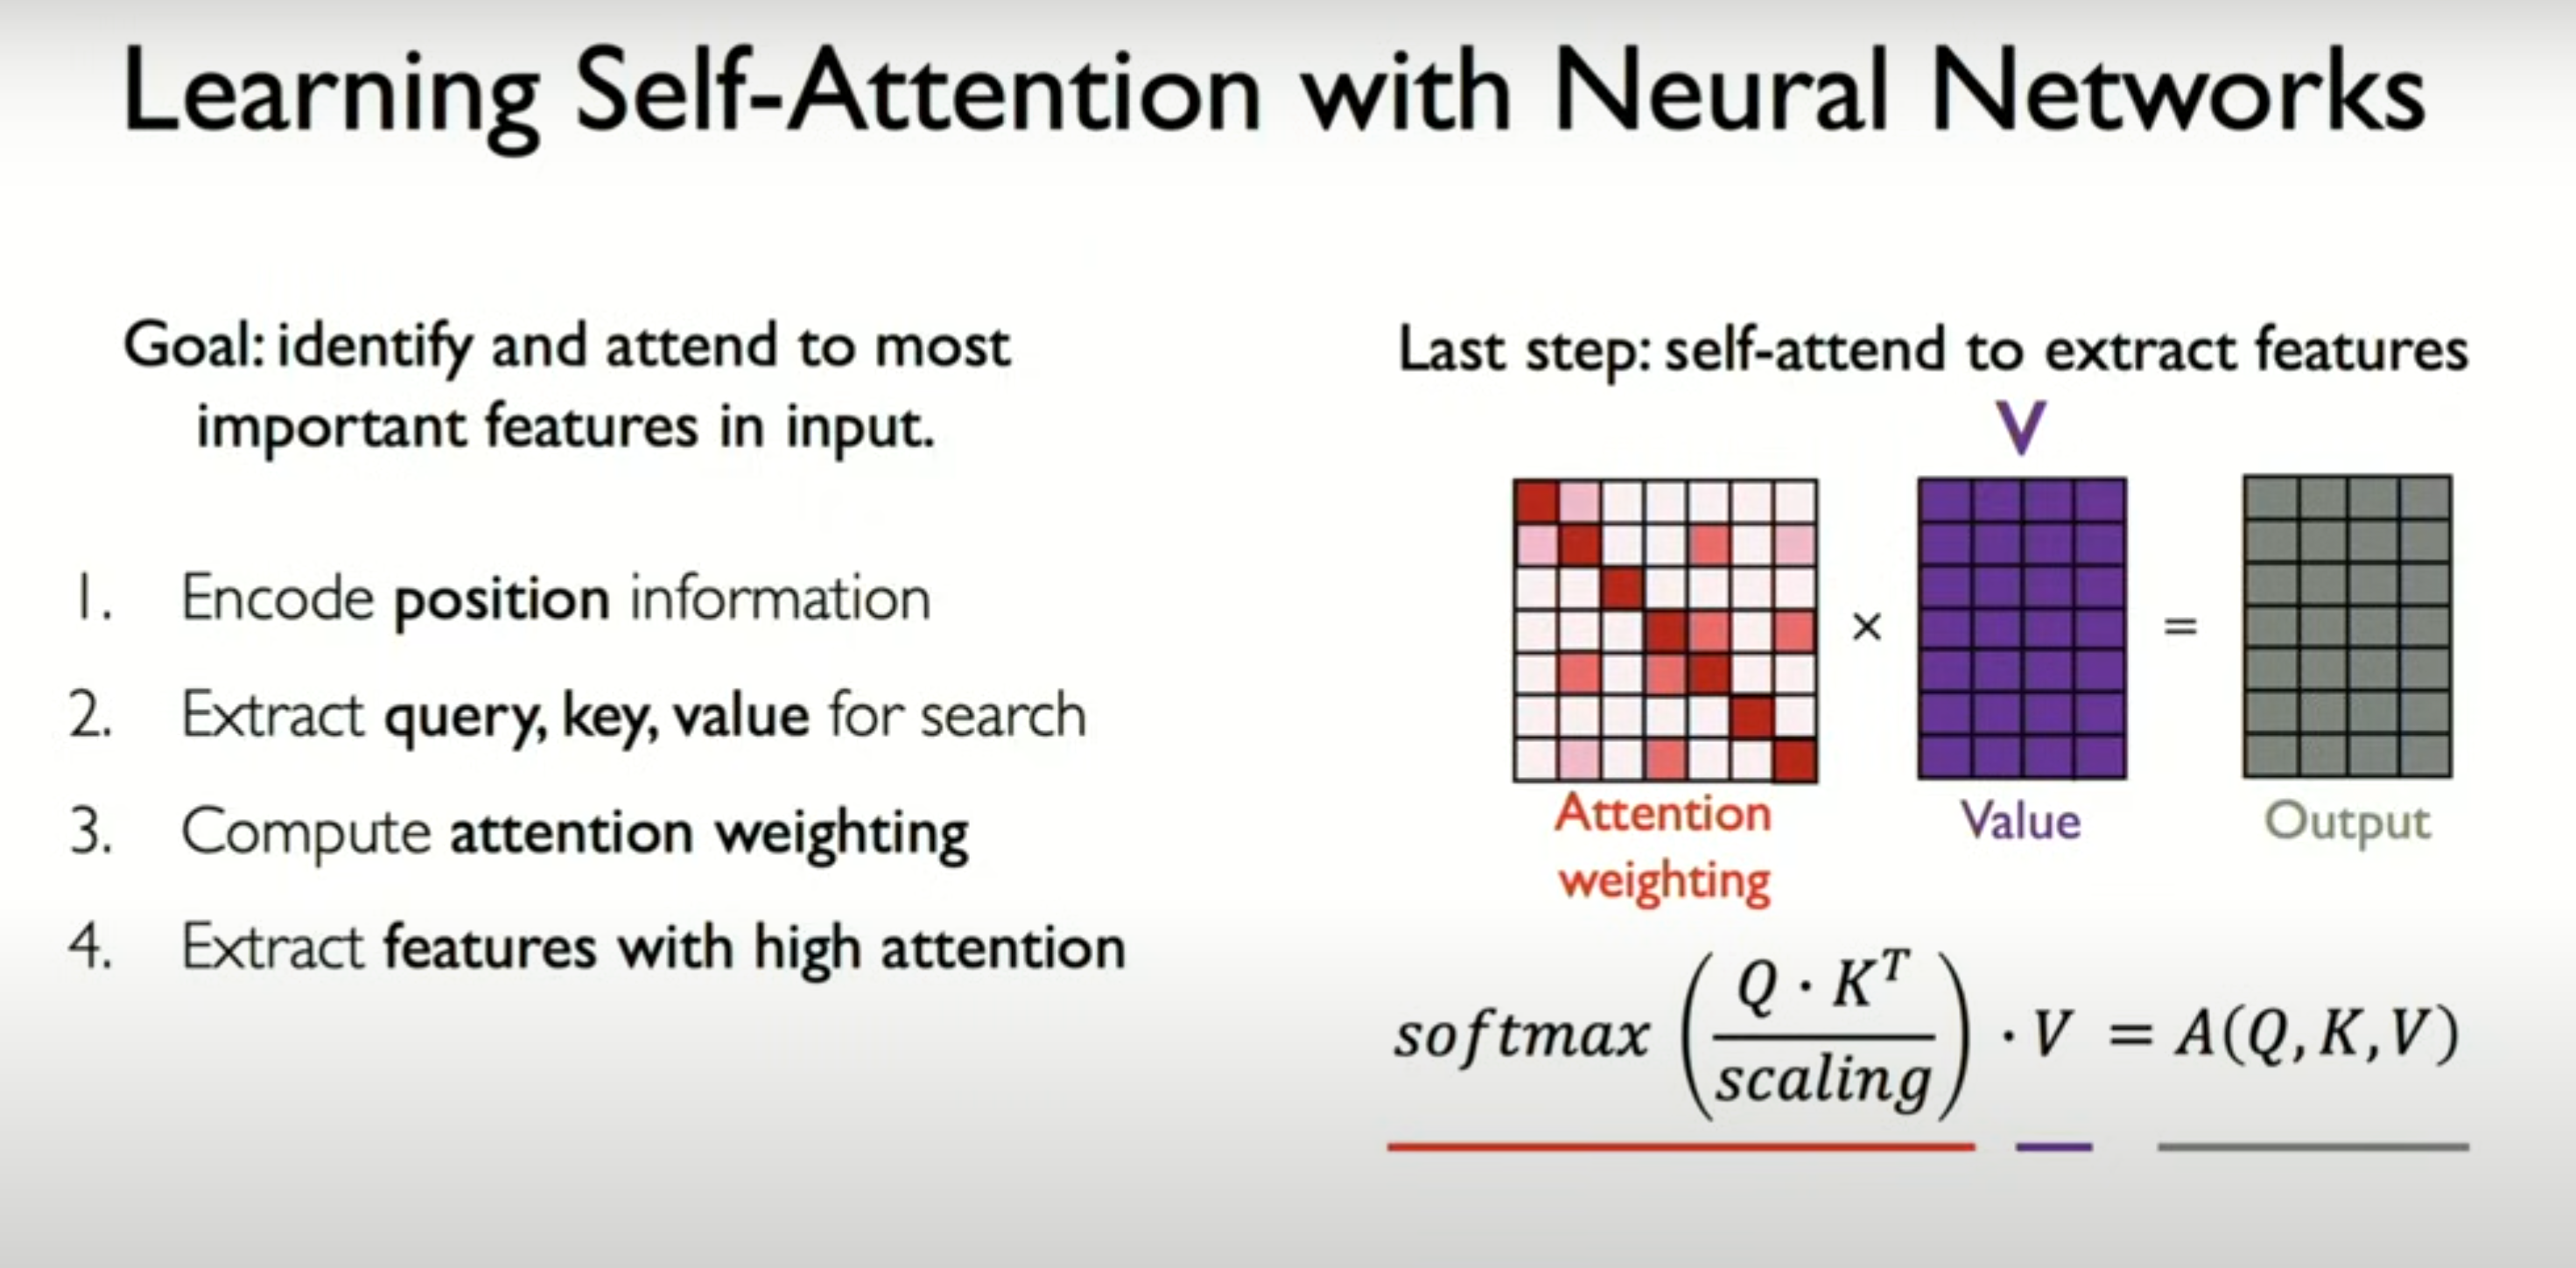
\includegraphics[width = 0.5\textwidth]{Images/attention_score3.png}
      \caption{Attention Score - Extracting the most important features}
    \end{figure}
    \item Now let's put it all together: 
    \begin{figure}[H]
      \centering
      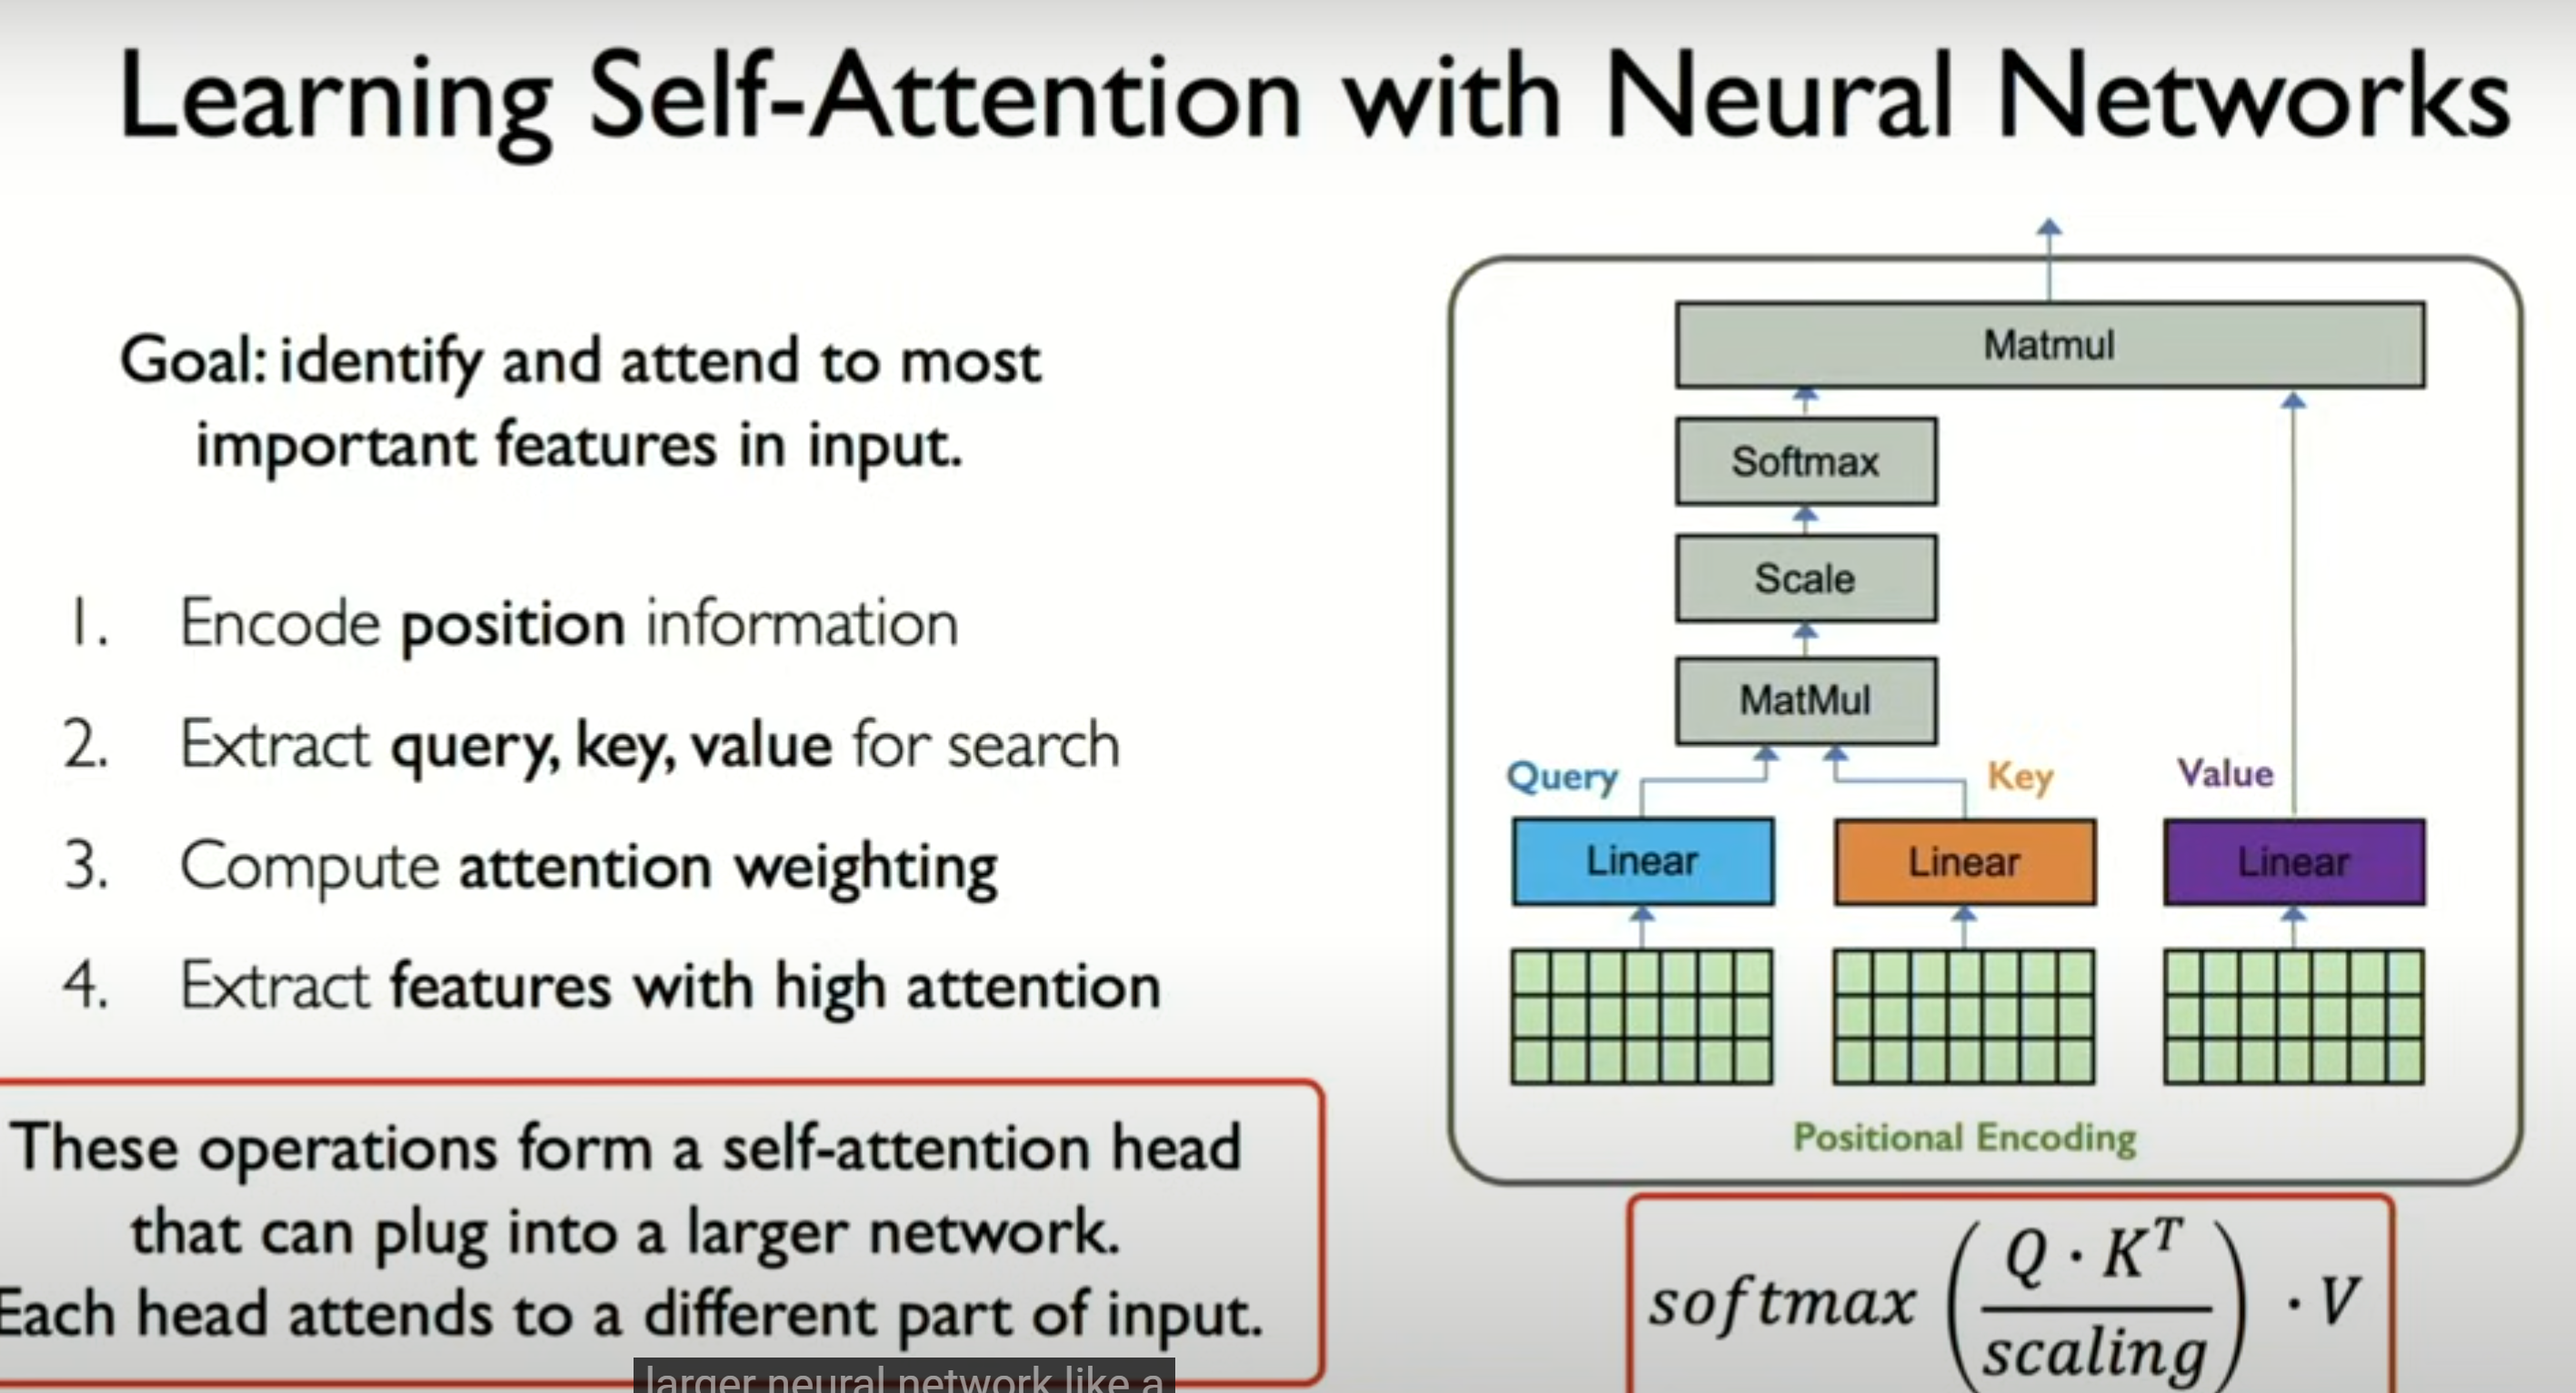
\includegraphics[width = 0.8\textwidth]{Images/all_.png}
      \caption{Single Self-Attention Head}
    \end{figure}
    \item How Self-Attention Works: \\ 
    \underline{Formulate Queries:}\\
    For each word, create a query vector that represents what that word wants to know from the rest of the sequence. \\
    \underline{Match Queries to Keys:} \\
    Compare the query with the keys of all words using the dot product. This comparison gives a similarity score for each word.\\
    \underline{Assign Attention Weights:} \\
    Use the similarity scores to assign weights to each word’s value. Higher similarity results in higher attention weights. \\ 
    \underline{Compute the Output:} \\ 
    Combine the values using the attention weights to form a context-aware output for the current word. \\
    \underline{Importance of Q, K, and V:} \\ 
    Query: Determines the focus or what information is needed.\\ 
    Key: Helps in matching relevant information in the sequence.\\ 
    Value: Provides the actual content that is used to generate the final output. \\ 
    \item So by computing $Q.K^T$ we are essentially getting a  k x k matrix where each element is the similarity between the query and the key. Then we use softmax which will keep the k x k matrix the same size but will normalize it. Then we multiply this by the V which is the value matrix to get the final output.
    \item Now the last question: How does this fit in the transformer architecture?
    \item Each attention head computes its own set of query (Q), key (K), and value (V) vectors by applying different linear transformations to the input embeddings.
    \item The attention head then calculates attention scores by comparing the query vector to all key vectors in the sequence, using the dot product. These scores are used to weight the value vectors.
    \item The attention head combines the weighted value vectors to produce an output. This output emphasizes the parts of the input that are most relevant according to the head’s specific focus. 
    \item In models like the Transformer, multiple self-attention heads are used in parallel. The outputs from all heads are combined (concatenated) and then passed through another linear layer to produce the final output of the self-attention mechanism.
    \item So key points to remember: \\
    \item Attention is the foundation of the transformer architecture, enabling the model to focus on different parts of the input sequence.
    \item Self-Attention Head: A single pathway that computes attention for a specific aspect of the input.
    \item Multi-Head Attention: Combines multiple self-attention heads to capture various relationships and dependencies in the data.
    \item Diversity of Focus: Each head in multi-head attention can focus on different parts or features of the input, providing a more comprehensive understanding.
    \begin{figure}[H]
      \centering
      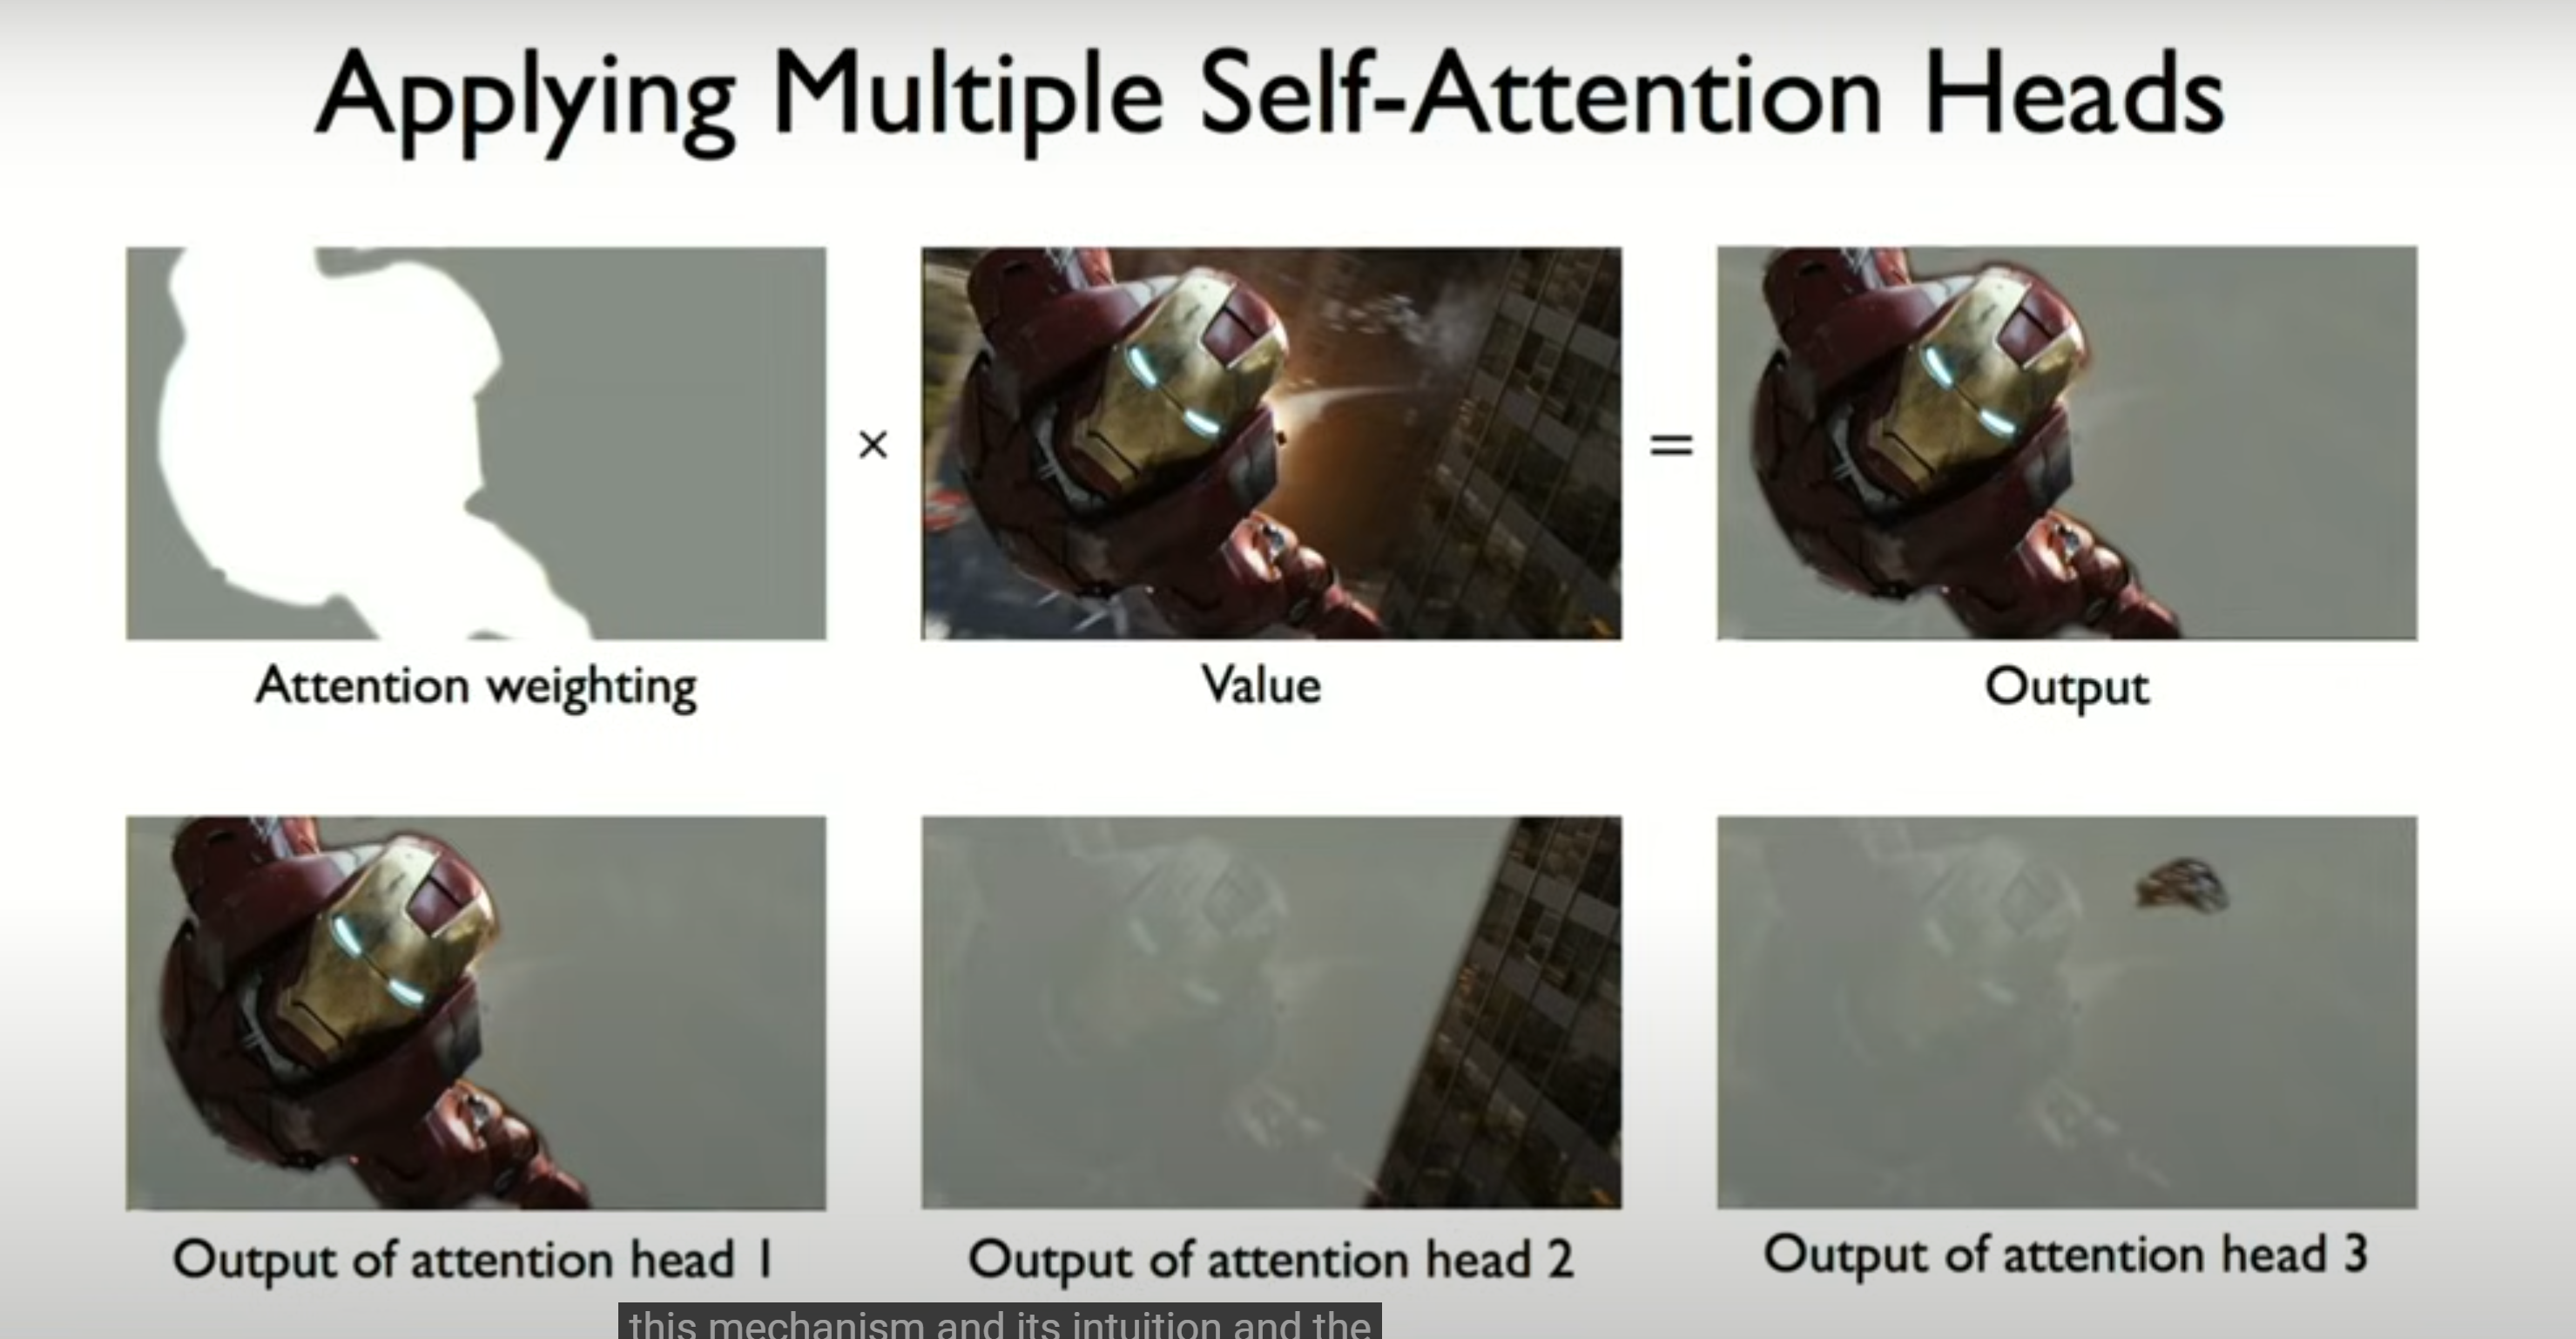
\includegraphics[width = \textwidth]{Images/multi_head.png}
      \caption{Multi Head Attention}
    \end{figure}
    \item We can see how in the first row we have the output of the softmax function, and then we multiply this by the value matrix to get the final output. (Which is what we need to focus on)
    \item We can see that each attention Head can be trained on focusing on a particular aspect of the input.
    \item Once we combine these self-attention heads we get the transformer architecture.
  \end{itemize}
\end{document}